%%%%%%%%%%%%%%%%%%%%%%%%%%%%%%%%%%%%%
%% Dissreta��o de Mestrado em Engenharia El�trica
%% Copyright 2009 Fabio de Oliveira Lima.
%% Este documento � distribu�do nos termos da licen�a 
%% GNU General Public License v2.
%%%%%%%%%%%%%%%%%%%%%%%%%%%%%%%%%%%%%

\documentclass[dvips,ruledheader, tocpage=plain, pagestart=firstchapter]{abnt}
\usepackage[latin1]{inputenc}
%\usepackage[num]{abntcite}
%\usepackage[alf]{abntcite}
\usepackage{abnt-alf}
\usepackage[dvips]{graphicx}
\usepackage[brazil]{babel}
\usepackage{srcltx}

% \usepackage{fullpage}
% \usepackage{color}
\usepackage{graphicx}
% \usepackage{epsfig}
% \usepackage{amsthm}
% \usepackage{latexsym}
\usepackage{amssymb}
%\usepackage{amsmath}
\usepackage{srcltx}

% Acrescentado por mim: CyberToddy

\usepackage[T1]{fontenc}
% \usepackage[latin1]{inputenc}
\usepackage[portuges]{babel}
% \sloppy

% example environment
% \newenvironment{example}
% {\emph{Exemplo:}}
% {\hfill $\boxtimes$\newline\newline}


\newcommand{\zz} {\vspace {0.3cm}} 
\newcommand{\z}{\par}
\newcommand{\bsq}{\z \hfill$\blacksquare$\zz}
\newcommand{\rr}{$^{\text{\textregistered}}$}
\newcommand{\Forall}[1]{,\forall\, \mbox{\small$#1$}}


\newenvironment{solucao}
{\emph{Solu��o:}}
{\hfill $\boxtimes$\newline\newline}

\newenvironment{dem}
{\emph{Demonstra��o:}}
{\bsq}

% some theorem environments
% \newtheorem{theorem}{Vari\'{a}vel}
% \newtheorem{proposition}{Dados}
% \newtheorem{claim}{Clamor}
% \newtheorem{lemma}{Lema}
% \newtheorem{corollary}{Corol\'{a}rio}


% \newtheorem{acknowledgement}[theorem]{Agradecimentos}
% \newtheorem{algorithm}[theorem]{Algoritmo}
% \newtheorem{axiom}[theorem]{Axioma}
% \newtheorem{case}[theorem]{Caso}
% \newtheorem{conclusion}[theorem]{Conclus\~{a}o}
% \newtheorem{condition}[theorem]{Conditi\c{c}\~{a}o}
% \newtheorem{conjecture}[theorem]{Conjectura}
% \newtheorem{criterion}[theorem]{Crit\'{e}rio}
\newtheorem{notation}{Notata\c{c}\~{a}o}
\newtheorem{data}{Dados}
\newtheorem{var}{Vari�vel}
% \newtheorem{problem}[theorem]{Problema}
% \newtheorem{remark}[theorem]{Observa\c{c}\~{a}o}
% \newtheorem{solution}[theorem]{Solu\c{c}\~{a}o}
% \newtheorem{summary}[theorem]{Sum\'{a}ario}

%\newenvironment{proof}[1][Proof]{\textbf{#1.} }{\ \rule{0.5em}{0.5em}}


% \newtheorem{definition}{Defini\c{c}\~{a}o} % Use this for non-trivial



% \usepackage{latexsym}
% \usepackage{psfrag}
% \usepackage[center]{caption2}

\usepackage{lineno}	% Numera as linhas.
% \linenumbers		% Numera as linhas, a partir do in�cio.
\pagewiselinenumbers	% Numera as linhas de cada p�gina.


\begin{document}
\citeoption{abnt-show-options=no}

%\DeclareGraphicsRule{.eps.gz}{eps}{.eps.bb}{`gunzip -c #1}


%% Capa
%% Copyright 2009 Fabio de Oliveira Lima.
%% Este documento � distribu�do nos termos da licen�a 
%% GNU General Public License v2.

% Usando o comando \capa

\titulo{UM MODELO EFICIENTE PARA O PROJETO COMPLETO DE REDES �PTICAS}

\autor{Fabio de Oliveira Lima}

\orientador{Prof. Dr. Elias Silva de Oliveira}
% ou \orientador[Orientadora:\\]{Minha orientadora}

\coorientador{Prof. Dr. Marcelo Eduardo Vieira Segatto}
% ou \coorientador[Co-orientadora:\\]{Minha co-orientadora}

\comentario{Disserta��o a ser apresentada � Coordena��o do Mestrado em Engenharia El�trica
 da Universidade Federal do Esp�rito Santo para a obten��o do t�tulo de Mestre em Inform�tica.}


\instituicao{Programa de P�s-Gradua��o em Engenharia El�trica \par 
	Centro de Tecnologia \par 
	Universidade Federal do Esp�rito Santo}

\local{Vit�ria -- ES}

\data{\today}

\capa

% ou...
% fazendo a mao
%
% \begin{titlepage}
%
%   ... codigo da folha de rosto
%  
% \end{titlepage}


% %%%%%%%%%%%%%%%%%%%%%%%%%%%%%%%%%%%%%
%%   Folha de rosto
%% Copyright 2009 Fabio de Oliveira Lima.
%% Este documento � distribu�do nos termos da licen�a 
%% GNU General Public License v2.
%%%%%%%%%%%%%%%%%%%%%%%%%%%%%%%%%%%%%

% Usando o comando \folhaderosto

\titulo{UM MODELO EFICIENTE PARA O PROJETO COMPLETO DE REDES �PTICAS}

\autor{Fabio de Oliveira Lima}

%  \begin{center}
%  Copyright 2009 Fabio de Oliveira Lima.\\ Este documento � distribu�do nos termos da licen�a \textbf{GNU} \textit{General Public License v2}.
%  \end{center}

\orientador{Prof. Dr. Elias Silva de Oliveira}
% ou \orientador[Orientadora:\\]{Minha orientadora}

\coorientador{Prof. Dr. Renato Tannure Rotta Almeida}
% ou \coorientador[Co-orientadora:\\]{Minha co-orientadora}

\comentario{Disserta��o apresentada ao Programa de P�s-Gradua��o em Engenharia El�trica do Centro Tecnol�gico da Universidade Federal do Esp�rito Santo,
como requisito parcial para obten��o do Grau de Mestre em Engenharia El�trica.}


\instituicao{Programa de P�s-Gradua��o em Engenharia El�trica \par 
	Centro Tecnologico \par 
	Universidade Federal do Esp�rito Santo}

\local{Vit�ria -- ES}

\data{\today}

\folhaderosto

% ou...
% fazendo a mao
%
% \begin{titlepage}
%
%   ... codigo da folha de rosto
%  
% \end{titlepage}


% %%%%%%%%%%%%%%%%%%%%%%%%%%%%%%%%%%%%%
%% Folha de Aprova��o
%% Copyright 2009 Fabio de Oliveira Lima.
%% Este documento � distribu�do nos termos da licen�a 
%% GNU General Public License v2.
%%%%%%%%%%%%%%%%%%%%%%%%%%%%%%%%%%%%%

\begin{folhadeaprovacao}
Disserta��o de Mestrado sob o t�tulo \textit{``UM MODELO EFICIENTE PARA O PROJETO COMPLETO DE REDES �PTICAS''}, a ser defendida por Fabio de Oliveira Lima e
aprovada em abril de 2010, em Vit�ria, Esp�rito Santo, pela banca examinadora constitu�da pelos doutores:

\setlength{\ABNTsignthickness}{0.4pt}
\setlength{\ABNTsignwidth}{10cm}
\setlength{\ABNTsignskip}{3cm}

\assinatura{Prof. Dr. Elias Silva de Oliveira \\ Departamento de Sistemas de Informa��o - UFES \\ Orientador}

\assinatura{Prof. Dr. Renato Tannure Rotta Almeida \\ Instituto Federal de Educa��o C\&T do Esp�rito Santo - Ifes \\ Coorientador}

% \assinatura{Prof. Dr. Marcelo Eduardo Vieira Segatto \\ Departamento de Engenharia El�trica - UFES \\ Examinador Interno}

\assinatura{Prof. Dr. Karcius Day Rosario Assis \\ Universidade Federal da Bahia \\ Departamento de Engenharia El�trica\\ Examinador Externo}

\end{folhadeaprovacao}


% %%%%%%%%%%%%%%%%%%%%%%%%%%%%%%%%%%%%%
%% Dedicatoria
%% Copyright 2009 Fabio de Oliveira Lima.
%% Este documento � distribu�do nos termos da licen�a 
%% GNU General Public License v2.
%%%%%%%%%%%%%%%%%%%%%%%%%%%%%%%%%%%%%


\pretextualchapter{}
\vfill

\begin{flushright}
\hfill \textit{Dedico esta disserta��o � minha esposa e ao meu filho}
\end{flushright}

\vspace*{1cm}

\clearpage


% Se comentado, cria um misterioso erro: n�o reconhesse o comando \chapter{}
%  
%% Agradecimentos
%% Copyright 2009 Fabio de Oliveira Lima.
%% Este documento é distribuído nos termos da licença 
%% GNU General Public License v2.


\chapter*{Agradecimentos}
\thispagestyle{empty}

\noindent Aos meus orientadores, pela oportunidade e pelos ensinamentos.% \\[10pt]

\noindent Aos meus familiares e amigos, por toda ajuda e apoio.

\noindent Aos desenvolvedores dos \textit{softwares} livres que utilizei.

\noindent Ao poder de s�ntese.

%%%%%%%%%%%%%%%%%%%%%%%%%%%%%%%%%%%%%%
%% Epigrafe
%% Copyright 2009 Marcelo de Oliveira Lima.
%% Este documento � distribu�do nos termos da licen�a 
%% GNU General Public License v2.
%%%%%%%%%%%%%%%%%%%%%%%%%%%%%%%%%%%%%


%  Ep�grafe - � uma cita��o pertinente ao seu trabalho
%  ou que represente o seu modo de pensar. 
%  Resumindo, coloque uma frase que o(a) agrade.


\pretextualchapter{}

\vspace{17.5cm}
\begin{flushright}

\textit{``A mente que se abre a uma nova id�ia jamais voltar� ao seu tamanho original.'' \\ 
	\bfseries Albert Einstein}

\end{flushright}




%%%%%%%%%%%%%%%%%%%%%%%%%%%%%%%%%%%%%
%% Resumo
%% Copyright 2009 Marcelo de Oliveira Lima.
%% Este documento � distribu�do nos termos da licen�a 
%% GNU General Public License v2.
%%%%%%%%%%%%%%%%%%%%%%%%%%%%%%%%%%%%%

\begin{resumo}

% Apresenta��o concisa dos pontos relevantes, dando uma visao rapida e
% clara do conte�do do trabalho.


 Este trabalho apresenta...

\end{resumo}


%%%%%%%%%%%%%%%%%%%%%%%%%%%%%%%%%%%%%%
%% Abstract
%% Copyright 2009 Fabio de Oliveira Lima.
%% Este documento � distribu�do nos termos da licen�a 
%% GNU General Public License v2.
%%%%%%%%%%%%%%%%%%%%%%%%%%%%%%%%%%%%%


\begin{abstract}

This paper presents a methodology for logical and physical design of optical communication networks with hierarchical topology of meshes. Are determined 
logical and physical topologies, and routing and designation of wavelengths, depending on the geographic location of network nodes. The methodology 
proposal consists of three steps that comprise a meta-heuristics, statistical inference and a model of mixed-integer linear programming. The first one 
genetic algorithm defines the hierarchical structure of the optical network. Then, a statistical procedure to obtain estimates 
parameters of interest that will be used to define quality criteria for the project, limiting the model variables 
mathematical programming resolved at the last step. We present results of experiments in order to validate the efficiency of this formulation on the 
computacinal performance and also regarding the quality of solutions, based on comparison of lower bounds for the metrics 
to be optimized. 

Keywords: optical networks, combinatorial optimization.

\textbf{\underline{Tradu��o GOOGLE!}}
\end{abstract}


\tableofcontents

% \listoffigures

% \listoftables


%%%%%%%%%%%%%%%%%%%%%%%%%%%%%%%%%%%%%
%% Introdu��o
%% Copyright 2009 Marcelo de Oliveira Lima.
%% Este documento � distribu�do nos termos da licen�a 
%% GNU General Public License v2.
%%%%%%%%%%%%%%%%%%%%%%%%%%%%%%%%%%%%%


\chapter{Introdu��o}
\label{intro}
\thispagestyle{empty}

A Multiplexa��o por Divis�o de Comprimentos de Onda (WDM), tecnologia que permite transmiss�o de v�rios sinais em diferentes comprimentos de onda
simultaneamente atrav�s de um mesmo enlace de fibra �ptica, juntamente com o Roteamento por Comprimento de Onda, realizado por n�s de rede que realizam o
roteamento dos sinais a partir do comprimento de onda dos mesmos, representam um alvo frequente de estudos nas �ltimas d�cadas.

Uma rede WDM consiste de n�s roteadores de comprimentos de onda interconectados atrav�s de enlaces ponto a ponto de fibra �ptica em uma determinada topologia.
Suas principais vantagens s�o o maior aproveitamento da largura de banda utilizada na fibra, menor custo relacionado ao processamento eletr�nico de dados nos
n�s da rede, transpar�ncia com rela��o ao protocolo de comunica��o e um eficiente tratamento/adequa��o a falhas dos componentes da rede, sejam falhas em enlaces
ou n�s. Com isso, as redes �pticas WDM com roteamento por comprimentos de onda (WRON) vem se consolidando como o padr�o de transmiss�o de dados em alta
velocidade.

Nas redes �pticas semi-transparentes \cite{ram96} parte do tr�fego a ser transmitido pela rede � transportado de maneira totalmente transparente
entre os pares de n�s que s�o interligados diretamente por caminhos �pticos. Entre os outros pares de n�s, s� � poss�vel o transporte de tr�fego atrav�s de
rotas formadas por mais de um caminho �ptico em seq��ncia. Neste segundo caso, o tr�fego deve ser processado nos n�s intermedi�rios de sua rota fonte-destino
para que  seja efetuada sua retransmiss�o pelo pr�ximo caminho �ptico. Ao se projetar redes WDM com roteamento de tr�fego por comprimento de onda, devemos
buscar uma solu��o que distribua e minimize o tr�fego alocado aos caminhos �pticos e tamb�m minimize o atraso m�dio de pacotes na rede.

Tradicionalmente o projeto de redes �pticas foi dividido em dois problemas que eram resolvidos de forma isolada \cite{ram96} \cite{murthy} \cite{mukherjee}
\cite{Karcius04}, s�o eles: Projeto da Topologia Virtual (VTD) e Roteamento e Aloca��o de Comprimentos de Onda (RWA). Nos �ltimos anos no entanto foram
apresentados na literatura abordagens integradas para os dois problemas \cite{Karcius04} \cite{Xin:03} e desta maneira o projeto de redes �pticas passou a ser
tratado de forma unificada, contemplando aspectos "f�sicos e virtuais" da rede. Os sub-problemas citados�s�o complexos e cada um deles � conhecido como
NP-Completo e a solu��o dos dois conjuntamente � ainda mais complexa. Diante disso, resolver o modelo matem�tico completo, em busca da solu��o �tima, torna-se
invi�vel. Como o objetivo � encontrar uma maneira de resolver o problema de forma integrada e com um tempo computacional�aceit�vel, o uso de de m�todos
(Meta-)Heur�sticos \cite{beas} torna-se uma boa alternativa.

\underline{\textbf{Falar de TWA, Hierarquia e teorias utilizadas...}}

A literatura recente mostra bons resultados para a estrat�gia descrita acima \cite{Karcius04} \cite{Xin:03}, ou seja, a utiliza��o de m�todos heur�sticos para
obter solu��es sub-�timas para o problema de projeto integrado de redes �pticas. Contudo, os estudos desenvolvidos at� aqui se concentraram em topologias em
malha. Para o presente trabalho de disserta��o a proposta � estender os resultados para topologias em hierarquias.

O restante deste texto est� organizado da seguinte forma: No Cap�tulo \\ref{} a seguir apresentamos.... No Cap�tulo \\ref{} � apresentada ... No Cap�tulo
\\ref{} s�o apresentados resultados computacionais obtidos....




%%%%%%%%%%%%%%%%%%%%%%%%%%%%%%%%%%%%%
%% Defini��o do Problema
%% Copyright 2009 Fabio de Oliveira Lima.
%% Este documento � distribu�do nos termos da licen�a 
%% GNU General Public License v2.
%%%%%%%%%%%%%%%%%%%%%%%%%%%%%%%%%%%%%


\chapter{Projeto de Redes �pticas Semitransparentes}
\label{vtd}

O projeto e planejamento de redes � realizado atrav�s de m�todos distintos de acordo com o tipo de tr�fego considerado, especificamente com rela��o a natureza
est�tica ou din�mica. No caso de tr�fego est�tico, nosso foco de estudo, � assumido \textit{a priori} uma determinada matriz de demanda de tr�fego,
representando a quantidade m�dia de tr�fego que deve ser transferido entre os pares de n�s da rede. Considera-se essas demandas como sendo fixas para fins
de planejamento, podendo
basear-se em levantamentos hist�ricos ou mesmo estudos estimativos. N�o ser�o consideradas aqui a possibilidade de bloqueio de pacotes e nem outros tipos de
perdas na transmiss�o. Portanto, � assumido que todo o tr�fego da rede ser� devidamente enviado e recebido.

Os canais �pticos transparentes entre os pares de n�s, por onde trafegam as demandas de tr�fego, chamados de liga��es l�gicas, formam a topologia
l�gica da rede. Entre o in�cio e o t�rmino de um caminho �ptico podem existir n�s intermedi�rios, pelos quais as demandas de tr�fego s�o roteadas de forma
transparente, isto �, no dom�nio �ptico. Por simplicidade, � assumido que todos as liga��es l�gicas possuem a mesma capacidade de tr�fego.

Todos os n�s da rede s�o equipados com OXCs (\textit{Optical Cross-Connect}) \cite{Zang00}. Cada caminho �ptico inicia e termina nos respectivos OXCs de seus n�s
de in�cio e t�rmino. O roteamento dos caminhos �pticos ao longo dos n�s da rede � realizado atrav�s dos OXCs dos n�s por onde eles passam.

N�o � considerada capacidade de convers�o de comprimentos de onda, dessa forma a restri��o de continuidade de comprimentos de onda deve ser respeitada. Dessa
forma, em todos as fibras por onde um caminho �ptico passa, ele deve utilizar o mesmo comprimento de onda.

A camada �ptica, que prov� caminhos �pticos �s camadas clientes, se tornou a principal camada de transmiss�o nos \textit{backbones} das redes de telecomunica��es.
Neste contexto, a camada �ptica pode ser vista como uma camada servidora e as que vem acima dela, fazendo uso dos servi�os oferecidos pela camada �ptica,
podem ser vistas como camadas cliente. 

Uma rede �ptica � transparente quando n�o existe convers�o eletr�nica dos caminhos �pticos durante o seu percurso fim-a-fim, enquanto uma rede �ptica �
opaca quando cada caminho �ptico � convetido eletronicamente em todos os n�s pelo qual transita na rede. Uma rede �ptica transparente n�o tem apenas
restri��es severas relacionadas com degrada��es acumuladas, mas tamb�m com monitora��o de performance, isola��o de falhas, gerenciamento centralizado,
continuidade de comprimento de onda entre outras \cite{bala00}. Usando redes �pticas semitransparentes, � poss�vel alcan�ar uma performance muito pr�xima
aos das redes opacas em termos de bloqueio de novas requisi��es, por�m com grande economia nos custos, e menos complexidade do que uma rede completamente
�ptica. Em suma, redes semitransparentes oferecem o melhor dos dom�nios �pticos e eletr�nicos sem comprometer as principais caracter�sticas de cada uma
dessas tecnologias \cite{bala00}.

\section{Projeto de Topologias L�gicas}

No estudo de formas eficientes de distribui��o de tr�fego em redes �pticas, uma caracter�stica da rede que influencia fortemente no resultado da 
distribui��o � a sua \textit{topologia}. A topologia l�gica \cite{ram02}, ou virtual, de uma rede �ptica � composta por caminhos �pticos que abstraem a
estrutura f�sica da rede, e pode ser representada por um grafo orientado \cite{cormen02}. Em redes WDM a topologia f�sica determina apenas o percurso f�sico
 dos caminhos �pticos. A topologia f�sica de uma rede �ptica pode ser representada por um grafo n�o orientado \cite{boaventura} onde os v�rtices
representam os n�s da rede e as arestas os enlaces f�sicos que unem estes n�s. 

O grau l�gico de entrada ou de sa�da de um n� � o n�mero m�ximo de enlaces l�gicos que podem se originar ou terminar nele, 
respectivamente. Fixado um valor de grau l�gico ($\Delta$) para a rede, todos os n�s dever�o ter o mesmo valor de grau l�gico de entrada e sa�da. Uma das
representa��es usuais para a topologia virtual de uma rede �ptica � sua matriz de adjac�ncias ($b$); uma matriz com entradas bin�rias, onde $b_{i,j}=1$, se
houver uma liga��o l�gica partindo do n� $i$ e terminando no n� $j$, e $b_{i,j}=0$ caso contr�rio. Entre os n�s origem e destino de uma liga��o l�gica podem
existir n�s e passagem, onde a conex�o do n� anterior e o posterior � feita de modo transparente, sem convers�o eletro-�ptica \cite{ram02}.

\begin{figure}[ht]
  \begin{center}
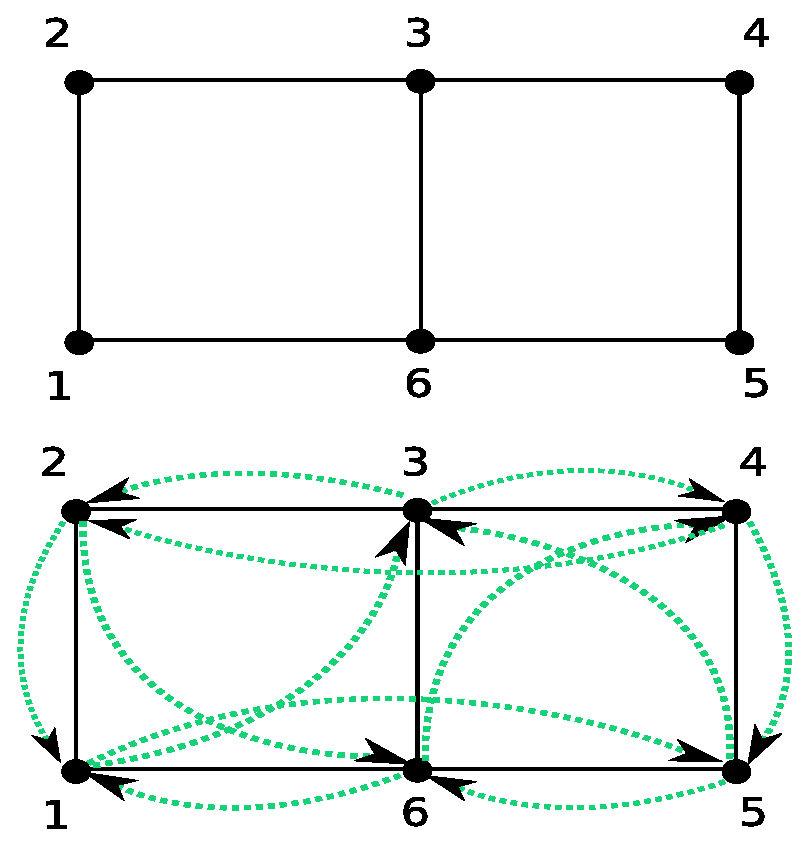
\includegraphics[scale=0.6]{figs/topologias.eps}
  \end{center}
  \caption{Exemplos para uma rede �ptica com 6 n�s. (a) Topologia f�sica. (b) Topologia virtual, com grau l�gico dois, nesta rede.}
  \label{topologias}
\end{figure}

\begin{figure}[htb]
  \begin{center}
\includegraphics[scale=0.6]{figs/2aneis.eps}
  \end{center}
  \caption{Exemplos, para uma rede �ptica com 4 n�s, de duas topologias em anel, com grau l�gico unit�rio.}
  \label{2aneis}
\end{figure}

 Na Figura \ref{topologias} temos o exemplo de uma topologia f�sica e uma topologia l�gica, para uma rede �ptica de seis n�s, com grau l�gico dois. Uma topologia
virtual conexa \cite{cormen02} de grau l�gico um � chamada de anel. Na Figura \ref{2aneis} encontramos exemplos de topologias virtuais em anel. 
A matriz de tr�fego $ \Lambda $, especifica as demandas de tr�fego $ \Lambda^{(s,d)} $ entre cada par fonte-destino $ (s,d) $ dos $n$ n�s da rede. Em geral, as
demandas de tr�fego $ \Lambda^{(s,d)} $ podem ser transportadas por mais de um caminho �ptico entre $ (s,d) $. E podem ser divididas em parcelas, utilizando
caminhos �pticos diferentes para escoar uma demanda. 

% A liga��o l�gica, entre dois n�s  $ (i,j) $, � aqui representada por $\alpha_{ij}$. A parcela de tr�fego, da uma demanda $ \Lambda^{(s,d)} $, passando por
% $\alpha_{ij}$ � chamada componente de tr�fego, � representada por $ \lambda_{ijsd} $.

Trabalhos realizados anteriormente apontam a mesma fun��o objetivo \cite{ram96} para este problema que estamos tratando; a minimiza��o do
congestionamento. O congestionamento � a quantidade de tr�fego designado ao caminho �ptico mais carregado da rede. Ao minimizar o congestionamento a
tend�ncia � distribuir igualmente o tr�fego entre todos os caminhos �pticos. Este crit�rio garante que n�o haja subutiliza��o ou sobrecarga nos enlaces l�gicos
que formam a topologia virtual da rede. A sobrecarga causa aumento do atraso em filas e consequente diminui��o do vaz�o \cite{ram02}.

O VTD consiste na determina��o de quais n�s ser�o interligados diretamente. A topologia virtual � base para a solu��o do problema de distribui��o de tr�fego. Uma
solu��o deste problema consiste em determinar uma topologia virtual e a forma como as demandas de tr�fego ser�o escoadas atrav�s da concatena��o dos diversos
caminhos �pticos. 


\section{Roteamento e Aloca��o de Comprimentos de Onda}

O roteamento e aloca��o de comprimentos de onda ou RWA, como � mais conhecido, pode ser definido como a seguir: dada a topologia f�sica de uma WRON e
um conjunto de requisi��es de conex�o l�gicas transparentes, selecione uma rota f�sica adequada para cada conex�o, com um determinado comprimento de onda,
de modo que n�o haja duas rotas alacadas a um mesmo comprimento de onda compartilhando a mesma liga��o f�sica ao longo do seu trajeto \cite{mukherjee}. Este
conjunto de requisi��es de conex�o nada mais � do que a topologia l�gica obtida como parte da solu��o do VTD.

\begin{figure}[htb]
 \centering
 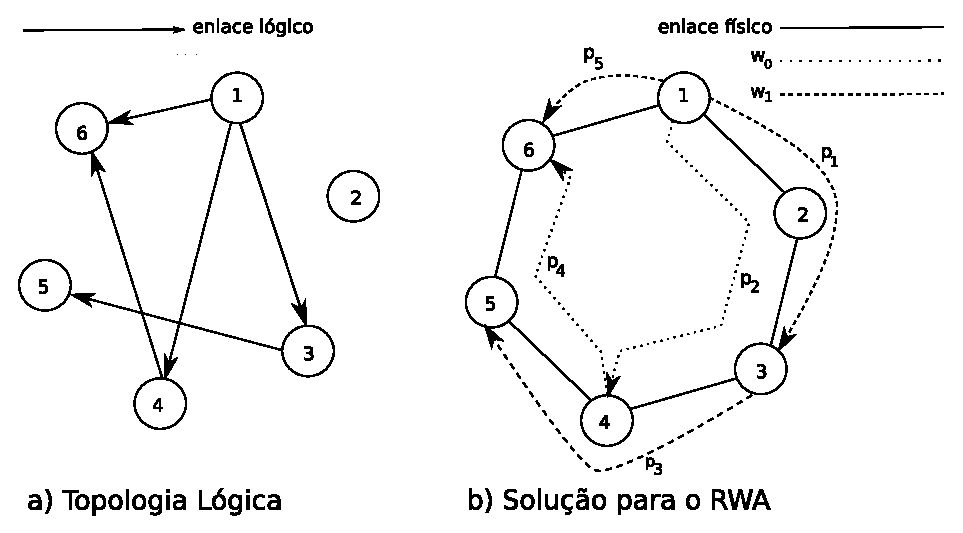
\includegraphics[bb=79 523 525 764]{figs/RWA.eps}
 % RWA.eps: 0x0 pixel, 300dpi, 0.00x0.00 cm, bb=79 523 525 764
 \caption{Exemplo de uma inst�ncia do RWA}
 \label{fig:rwa}
\end{figure}


Cabe aqui observar que estamos modelando a topologia
f�sica como um grafo direcionado. Deste modo, duas conex�es l�gicas cujos trajetos alocados passam por uma mesma liga��o f�sica $(m,n)$, mas em sentidos
opostos, est�o necessariamente em fibras distintas, satisfazendo assim esta defini��o.  

Na figura \ref{fig:rwa} temos uma exemplo de uma inst�ncia para o RWA, onde um dos dados de entrada � a topologia l�gica obtida do VTD. A solu��o obtida
apresenta os
percursos por onde ser�o roteadas as liga��es l�gicas com os comprimentos de onda escolhidos.

O objetivo mais comum � minimizar o n�mero de comprimentos de onda necess�rios para estabelecer uma certa configura��o de caminhos �pticos para uma dada
topologia
f�sica \cite{mukherjee}. Uma alternativa � minimiza��o de comprimentos de onda � maximizar o n�mero de conex�es que podem ser estabelecidas para um dado
n�mero de comprimentos de
onda e um dado conjunto de requisi��es de conex�o \cite{Zang00}. 




 



















%%%%%%%%%%%%%%%%%%%%%%%%%%%%%%%%%%%%%
%% Revis�o Bibliogr�fica
%% Copyright 2009 Fabio de Oliveira Lima.
%% Este documento � distribu�do nos termos da licen�a 
%% GNU General Public License v2.
%%%%%%%%%%%%%%%%%%%%%%%%%%%%%%%%%%%%%


\chapter{Trabalhos Anteriores}

O problema de projetar uma rede �ptica, a partir de uma topologia f�sica conhecida, pode ser formulado como um problema de programa��o inteira mista (MILP
- \textit{Mixed Integer Linear Problem}), sendo definida uma m�trica de interesse a ser otimizada. Esse problema j� foi amplamente  estudado, tendo sido
propostas heur�sticas para resolv�-lo, sendo conhecidamente um priblema de alto custo computacional \cite{Sivarajan01,Xin:03}. As diferentes abordagens
partem de considera��es espec�ficas sobre as demandas de tr�fego, a m�trica a ser otimizada, entre outras. O objetivo normalmente � a minimiza��o de algum
recurso da rede, tendo como exemplos: n�mero de comprimentos de onda utilizados, n�mero de transceptores, congestionamento e processamento eletr�nico.

Uma das formula��es para o projeto de uma topologia virtual foi apresentado como um problema de otimiza��o em \cite{Mukherjee96}. Os autores formularam o
problema de projeto de topologia l�gica como um problema de otimiza��o n�o linear. A fun��o objetivo considerava a minimiza��o do atraso na transmiss�o e do
congestionamento da rede. Os autores subdividem o problema em quatro subproblemas, da forma como foi mostrada na Se��o \ref{4sub}. Nos experimentos
apresentados, os autores consideram apenas o VTD, subproblemas LTD e TR. A meta-heur�stica \textit{Simulated annealing} foi utilizada na resolu��o do
subproblema LTD e \textit{flow deviation} para o subproblema TR. Entretando, a meta-heur�stica \textit{Simulated Annealing} implementada torna-se muito cara
computacionalmente para redes de grands porte.

Em \cite{Banerjee00} � apresentada uma forma��o MILP para o projeto completo de uma WRON com convers�o de comprimentos de onda. Vale ressaltar que, em redes
equipadas com conversores de comprimentos de onda, o problema torna-se menos complexo pois a restri��o de continuidade dos comprimentos de onda n�o �
aplicada \cite{Zang00}. O objetivo neste trabalho era minimizar a dist�ncia m�dia das rotas f�sicas. A formula��o MILP apresentada, inclui a defini��o das
liga��es l�gicas, suas rotas f�sicas, e a distribui��o de tr�fego sobre as mesmas. Com o objetivo de tornar o problema trat�vel, a restri��o de continuidade
de comprimentos de onda foi relaxada, considerando que todos os n� possuem capacidade de convers�o de comprimentos de onda. Devido � dificuldade de obter
solu��es �timas com o modelo MILP o processo de otimiza��o foi interrompido ap�s algumas itera��es.

Em \cite{ram96} os autores formularam uma modelagem MILP para o VTD com o objetivo principal de minimizar congestionamento. N�o existe restri��o
quanto ao n�mero de comprimentos de onda utilizados. A desvantagem desta abordagem � que a topologia f�sica torna-se irrelevante para o projeto, pois ela �
considerada apenas para limtar o atrazo de propaga��o. A estrutura f�sica influencia muito pouco dessa forma. Al�m disso, o atrazo � calculado supondo que
as rotas f�sicas s�o estabelcidas pelo algoritmo da menor dist�ncia \cite{Zang00}.

Em \cite{Sivarajan01} � proposta uma modelagem MILP que minimiza congestionamento em redes sem conversores de comprimentos de onda. Segundo os autores, esta
formula��o n�o � computacionalmente trat�vel, sendo m�todos heur�sticos propostos. O Modelo MILP � relaxado e executado interativamente por $25$ vezes usando um
plano de corte. As vari�veis que representam a topologia virtual e os percursos f�sicos s�o arredondadas, enquanto uma heur�stica de aloca��o de comprimentos de
onda � aplicada para atribuir-los individualmente �s rotas f�sicas. Uma das desvantagens desse m�todo � que, supondo que existam $W$ comprimentos de onda
dispon�veis em cada fibra, o algoritmo de aloca��o de comprimentos de onda pode n�o garante sucesso. Em caso de falha, ele ser� reiniciado incrementando
$W$. Como resultado, o m�todo n�o retorna necessariamente solu��es vi�veis em todas as tentativas.

Em \cite{Banerjee97}, os autores formularam o problema de projeto de topologia l�gica como um problema linear que considera os n�s da rede equipados com
conversores de comprimento de onda. A fun��o objetivo da formula��o � a minimiza��o do comprimento das rotas f�sicas, com a possibilidade de
redu��o do n�mero de conversores de comprimentos de onda utilizados e, dessa forma, esta formula��o poderia ser aproximada para uma formula��o sem
convers�o. As defici�ncias desta formula��o s�o: ela produz resultados razo�veis somente se a matriz de tr�fego for equilibrada, sendo esta uma
consequ�ncia da fun��o objetivo n�o incluir vari�veis de tr�fego; ele � eficiente somente se a topologia f�sica for densa em termos do n�mero de arestas.
Se a topologia f�sica for esparsa ent�o o n�mero de conversores de comprimento de onda utilizados aumentar�, pois haveriam poucas rotas auternativas. A
restri��o de continuidade dos comprimentos de onda n�o foi utilizada nesta formula��o.

O artigo \cite{Tornatore07} apresenta um modelo MILP para o projeto de WRONs, capaz de projetar tamb�m a rede f�sica, suportando m�ltiplos cabos de fibra
�ptica entre cada par n�s. No modelo proposto � usada agrega��o de v�ri�veis em rela��o � origem para a cria��o das rotas f�sicas, o que permite uma redu��o
relevante no n�mero de vari�veis e restri��es \cite{Jaumard04}. Com rela��o a convers�o de comprimentos de onda, dois casos extremos s�o tratados: 1) quando
todos os n�s possuem capacidade de converter os comprimentos de onda, e 2) quando nenhum n� possui capacidade de convers�o de comprimento de onda, sendo
exigida a restri��o de continuidade de comprimentos de onda. O trabalho prop�e a otimiza��o da topologia l�gica de uma rede f�sica com m�ltiplos
cabos de fibras entre os pares de n�s, com o objetivo de minimiza��o de custo: o n�mero de liga��es f�sicas entre cada par de n�s � a vari�vel a ser
minimizada, tendo como um dos dados de entrada o n�mero de comprimentos de onda por liga��o f�sica. 

Algumas heur�sticas para o projeto completo de redes �pticas foram apresentadas no artigo \cite{Nina05}, aplicando o modelo proposto em \cite{Sivarajan01}.
Este trabalho envolve o projeto de WRONs sem utiliza��o de conversores de comprimento de onda. Neste trabalho � introduzida uma fun��o objetivo chamada, o
numero m�dio de saltos l�gicos (\textit{average virtual hop distance}), onde o n�mero de saltos l�gicos � a quantidade de liga��es l�gicas que por onde uma
demanda de tr�fego passa antes de chagar ao destino. As heur�sticas apresentadas s�o adapta��es das apresentadas em \cite{ram96}. Os resultados apresentados
foram gerados a partir de experimentos com redes de tamanhos variados e para caracter�sticas de tr�fego uniforme e n�o uniforme.

Uma refer�ncia cl�ssica para o RWA � o artigo \cite{Zang00}. Este estudo detalha o problema de roteamento e aloca��o de comprimentos de onda (RWA) em redes
�pticas WDM, especialmente para redes que operam com
a restri��o de continuidade de comprimentos de onda, ou seja, n�o utilizam conversores. � apresentada uma revis�o de v�rias abordagens e m�todos apresentadas na
literatura, abrangendo modelagens MILP e heur�sticas.

Um modelo MILP para o projeto completo foi apresentado em \cite{Karcius04}, baseado nas formula��es cl�ssicas do VTD e do RWA. Este trabalho prop�e um
algoritmo heur�stico iterativo, que faz uso de programa��o linear, para resolver os problemas VTD e RWA de forma integrada. A topologia l�gica �
escolhida com a cl�ssica heur�stica HLDA \cite{ram96}, e esse resultado � fixado no modelo proposto. A seguir o modelo � resolvido para encontrar solu��o
para as demias vari�veis. Por se tratar de um modelo MILP de alto custo computacional, a resolu��o � interrompida depois de um tempo pr� determinado.
A fun��o objetivo adotada foi o n�mero total de saltos nas rotas f�sicas, com o objetivo de evitar a forma��o de ciclos nas rotas f�sicas. A estrat�gia foi
passar ao modelo limita��es para as m�tricas importantes, de modo que as solu��es vi�veis encontradas fossem satisfat�rias. Essa abordagem foi poss�vel
dada a grande abrang�ncia do modelo proposto, onde m�tricas dos quatro sub-problemas do projeto de uma WRON podem ser controladas. Todavia o alto custo
computacional do modelo proposto inviabiliza sua aplica��o para redes de grande porte. As redes testadas tinham $6$ e $12$ n�s.





%%%%%%%%%%%%%%%%%%%%%%%%%%%%%%%%%%%%%
%% Modelagem TWA
%% Copyright 2009 Fabio de Oliveira Lima.
%% Este documento � distribu�do nos termos da licen�a 
%% GNU General Public License v2.
%%%%%%%%%%%%%%%%%%%%%%%%%%%%%%%%%%%%%


\chapter{TWA - Modelo para o Projeto Completo de uma WRON }
\label{Basic}

Neste cap�tulo ser� apresentada a forma b�sica do modelo TWA (\textit{Traffic over Wavelength Assignment}), come�ando pela nota��o designada aos n�s e as
constantes que definem uma inst�ncia de
problema para o modelo. Em seguida ser�o definidas as vari�veis utilizadas para compor as restri��es e a fun��o objetivo do modelo, passando-se
ent�o � sua descri��o. A fun��o objetivo adotada na formula��o b�sica � a minimiza��o dos custos de instala��o e opera��o da rede, valendo-se da capacidade do
modelo escolher tamb�m a topologia f�sica da rede. Al�m disso, foi
considerada a restri��o de conserva��o dos comprimentos de onda ao longo do caminho �ptico \cite{Zang00}, ou seja, n�o se admite a convers�o de comprimentos de
onda na camada �ptica da rede nesta formula��o b�sica. Outros casos de uso e extens�es ao modelo b�sico ser�o apresentados no Cap�tulo \ref{cases}.

\section{Dados de Entrada e Vari�veis}

\begin{notation}
Para uma rede de $N$ n�s, os pares ordenados $(m,n)$, $(s,d)$ e $(i,j)$ indicam respectivamente liga��es f�sicas, demandas de tr�fego e liga��es l�gicas,
com $m\neq n$, $s\neq d$ e $i\neq j$, onde $m,n,s,d,i,j\in \{1,..,N\}$. O �ndice $w \in \{1,..,W\}$ representa comprimentos de onda, onde $W$ � a quantidade
limite de comprimentos de onda que podem ser usados. O �ndice $v\in \{1,..,N\}$ representa os n�s da rede.
\end{notation}

\begin{figure}[htb]
\centering
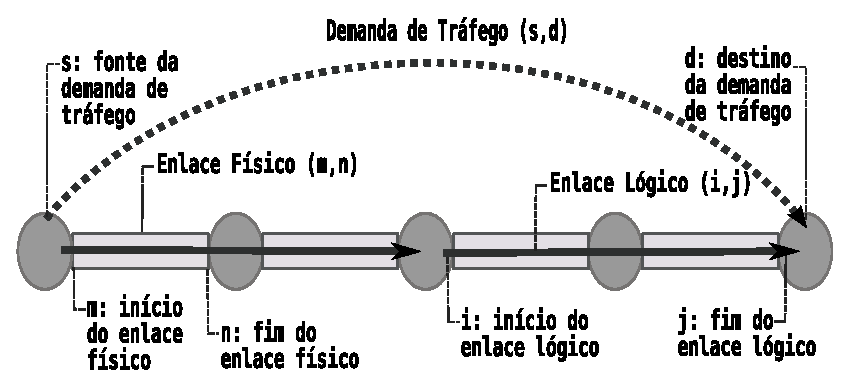
\includegraphics[bb=43 653 523 825,scale=.9]{figs/indices.eps}
\caption{Representa��o gr�fica da nota��o associada aos n�s da rede.}
\label{fig:Indices}
\end{figure}

A Figura \ref{fig:Indices} ilustra os diferentes escopos dos �ndices associados aos n�s da rede, com rela��o �s liga��es f�sicas $(m,n)$, liga��es l�gicas
$(i,j)$ e demandas de tr�fego $(s,d)$. Esta nota��o segue a conven��o comumente utilizada em trabalhos anteriores \cite{mukherjee,ram02}. �
importante dizer que esta modelagem suporta m�ltiplas liga��es f�sicas e l�gicas entre cada par de n�s, portanto, os pares $(m,n)$ e $(i,j)$ representam
conjuntos de poss�veis liga��es f�sicas e l�gicas, respectivamente. Esses conjuntos n�o ser�o explicitamente controlados, sendo esse um dos motivos
da simplicidade do modelo.

\begin{dados}
\label{Cons}
Uma inst�ncia para o modelo TWA � definida por:

\begin{enumerate}
\item $N$ $=$ N�mero de n�s da rede.
\item $W$ $=$ M�ximo de comprimentos de onda em uma liga��o f�sica.
% \item $H$ $=$ Grau f�sico m�ximo de entrada e sa�da de cada n�.
\item $K$ $=$ M�xima multiplicidade de liga��es f�sicas entre cada par $(m,n)$.
\item $Cap$ $=$ Capacidade de tr�fego de cada liga��o l�gica.
\item $C_{mn}$ $=$ Custo de uma liga��o f�sica entre o par $(m,n)$.
\item $T$ $=$ Custo por unidade de fluxo.
\item $P_{sd}$ $=$ Demanda de tr�fego, com origem $s$ e destino $d$.
\item $A_s = \sum_d P_{sd} =$ Tr�fego agregado pela origem $s$. 
\item $Q_{sd}=P_{sd}/A_s =$ Fra��o de $A_s$ correspondente � Demanda de tr�fego $P_{sd}$.
\end{enumerate}
\end{dados}

% \clearpage

 \subsection{Componentes Topol�gicos}
% \label{Top}

A vari�vel central do modelo, a partir da qual todas as demais ser�o definidas, chamada de componente topol�gico, � representada graficamente na Figura
\ref{fig:B} e formalmente definida na Vari�vel \ref{comp}. Ela sozinha representa as topologias l�gica e f�sica, as rotas f�sicas das 
liga��es l�gicas e os comprimentos de onda utilizados.

\begin{var}
\label{comp}
 Seja $B_{iw}^{mn} = k\in \{0,..,K\}$, com $i\neq n$, um componente do conjunto das liga��es l�gicas com origem $i$ e comprimento de onda $w$,
que utilizam $k$ liga��es f�sicas entre os n�s $m$ e $n$.
\end{var}

\begin{figure}[hbt]
 \centering
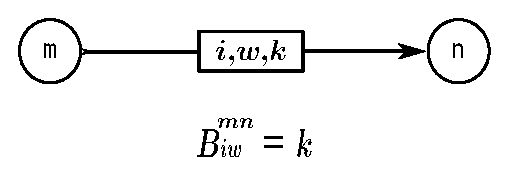
\includegraphics[bb=177 683 405 753, scale=0.9]{figs/B.eps}
% B.eps: 1179666x1179666 pixel, 300dpi, 9987.84x9987.84 cm, bb=36 739 246 805
 \caption{Representa��o gr�fica de um componente topol�gico.}
 \label{fig:B}
\end{figure}

Considerando que $B_{iw}^{mn}=k$ para algum $k \in \{0,..,K\}$, existem $k$ liga��es l�gicas originadas em $i$ no comprimento de onda $w$, passando
por $k$ liga��es f�sicas distintas entre o par de n�s $(m,n)$.  Conforme a terminologia utilizada
neste trabalho daqui por diante, \textit{um componente topol�gico $B_{iw}^{mn} = k$ � iniciado em $m$, incidente em $n$, com origem $i$,
comprimento de onda $w$ e valor $k$}.

Se $k>1$, ent�o h� multiplicidade de liga��es f�sicas entre o par de n�s $(m,n)$,
pois haveria interfer�ncia se houvessem duas liga��es l�gicas se propagando na mesma liga��o f�sica, com o mesmo comprimento de onda. Note
que $K$ limita apenas a multiplicidade das liga��es f�sicas, pois se $K=1$, $B_{iw}^{mn}$ se torna uma vari�vel bin�ria, mas ainda podem haver m�ltiplas
liga��es l�gicas entre um par $(i,j)$, utilizando rotas f�sicas distintas, ou ainda, comprimentos de onda diferentes em uma mesma
rota f�sica. Se $B_{iw}^{mn}=0$, $\forall\,(i,w)$, ent�o nenhuma liga��o f�sica entre o par de n�s $(m,n)$ � utilizada.

 Na Figura \ref{fig:Tops}, temos um exemplo de interpreta��o dos componentes topol�gicos, todos com origem no n� $v_1$ e com o 
mesmo comprimento de onda $w_1$. No item $d)$ desta figura, o valor $2$ do componente que liga os n�s $(v_1,v_2)$ � interpretado 
como duas liga��es f�sicas entre esses n�s, representadas no item $a)$. No item $b)$, vemos uma liga��o l�gica dupla entre os 
n�s $(v_1,v_3)$, onde uma delas passa de forma transparente pelo n� $v_2$, como indicado no item $c)$. Note ainda que, no item 
$d)$, h� dois caminhos l�gicos incidentes em $v_2$ mas apenas um iniciando. Isso indica que uma liga��o l�gica termina em $v_2$, 
enquanto a outra segue adiante.

% \clearpage
\begin{figure}[hbt]
 \centering
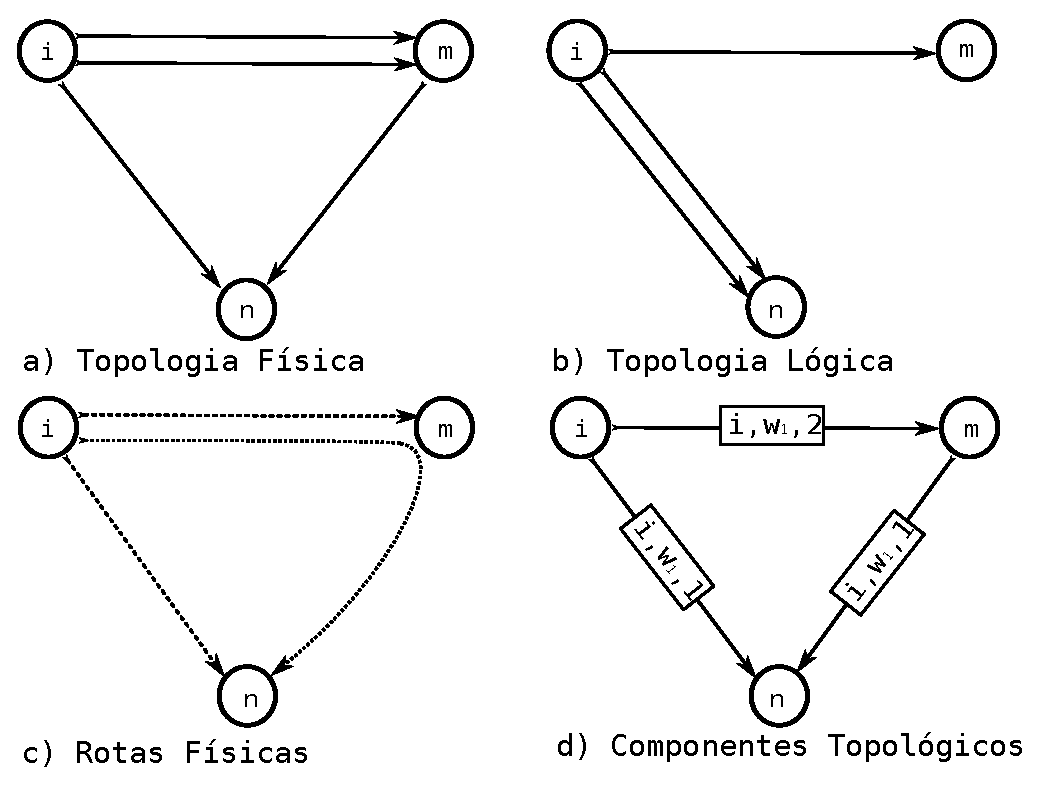
\includegraphics[width=0.8\textwidth]{figs/topologias-twa.eps}
% 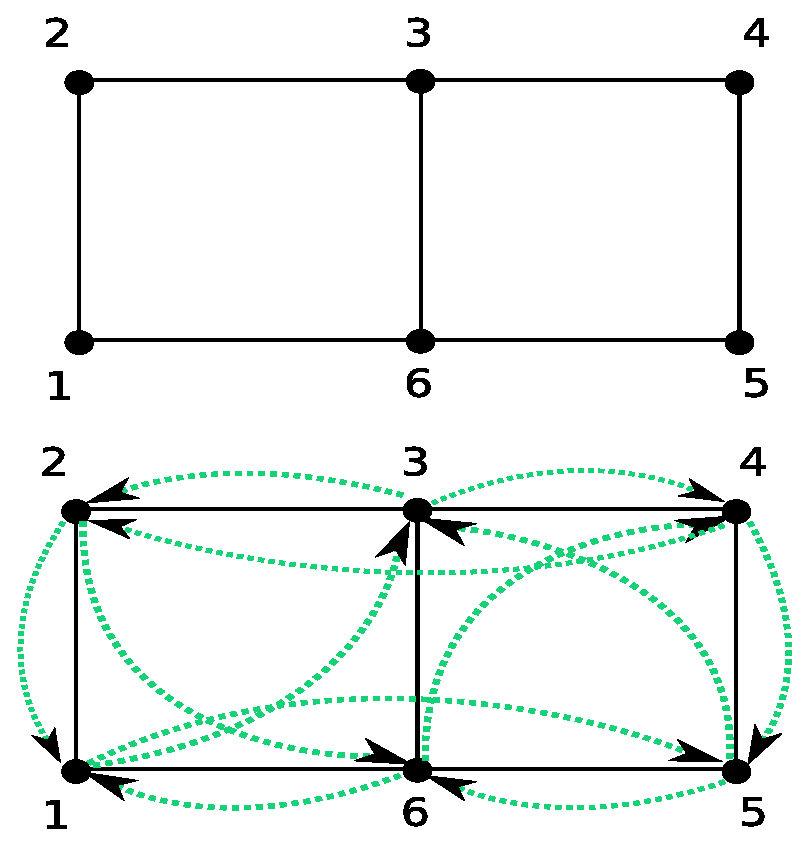
\includegraphics[bb=39 455 511 811, scale=0.4]{figs/topologias.eps}
 % topologias.eps: 1179666x1179666 pixel, 300dpi, 9987.84x9987.84 cm, bb=30 375 511 801
 \caption{Exemplo da interpreta��o dos componentes topol�gicos.}
 \label{fig:Tops}
\end{figure}
% \clearpage

A indexa��o atribu�da �s vari�veis $B_{iw}^{mn}$ especificam apenas o n� $i$ onde se iniciam as liga��es l�gicas representadas, sem deixar claro
aonde elas terminam. Isto significa que estas vari�veis agregam todas as liga��es l�gicas originadas em $i$ com comprimento de onda $w$, que utilizam as
liga��es f�sicas entre o par $(m,n)$, independente do n� $j$ em que terminam estas liga��es l�gicas. Esta t�cnica consiste em uma abordagem bastante
conhecida para a representa��o de vari�veis em problemas de distribui��o de fluxo em redes. Em \cite{Tornatore07}, este conceito de agrega��o de tr�fego �
aplicado como meio de simplifica��o do modelo, reduzindo substancialmente o n�mero de vari�veis dos problemas resultantes. No TWA, esta agrega��o cumpre o
mesmo papel de simplifica��o, cabendo �s restri��es do modelo garantir implicitamente a termina��o correta destas liga��es l�gicas agregadas nas vari�veis
$B_{iw}^{mn}$.

Para fins de compara��o entre modelos de programa��o inteira, usualmente uma vari�vel que pode assumir $K$
valores diferentes � convertida em $K$ vari�veis bin�rias \cite{cormen02}. A princ�pio, o n�mero de vari�veis bin�rias associadas aos componentes
topol�gicos seria $N^3\cdotp W\cdotp K$ \cite{cormen02}, mas devemos excluir algumas que s�o trivialmente nulas: aquelas com $i=n$, pois $i$ n�o pode ser
origem da liga��o l�gica e ao mesmo tempo destino da liga��o f�sica ($n$). Isso resulta em $N^3\cdotp W\cdotp K - N^2\cdotp K$.


\subsection{Fra��o de Fluxo das Demandas de Tr�fego}
\label{cap:twa-sec:VarFracFlow}

Para resolver o sub-problema de roteamento de tr�fego, � definida a vari�vel Vari�vel \ref{FlowVar}, que modela a fra��o de fluxo agregado para as
demandas de tr�fego. Elas s�o
semelhantes �s vari�veis de fluxo agregado utilizadas em \cite{ram96}, todavia h� duas diferen�as. Uma delas � que aqui essas vari�veis s�o normalizadas em
fun��o do tr�fego agregado na origem ($A_s$), e s�o portanto uma fra��o deste. Essa modifica��o n�o � requerida pela modelagem, tendo apenas a fun��o de
facilitar a compreens�o das restri��es do modelo, que ficam menos dependentes do dados de entrada. 

A outra diferen�a � que o fluxo � separado por comprimento de onda, como se fossem $W$ redes sem multiplexa��o sobrepostas. Isso facilita a interpreta��o
das
restri��es do modelo, e tamb�m ajuda a mant�-lo mais simples. De fato, o controle da distribui��o de fluxo deve ser feito em cada liga��o l�gica
\cite{ram02}, mas a restri��o de continuidade de comprimentos de onda exige uma equa��o para cada $w$ separadamente \cite{Zang00}. Soma-se a isso o fato de
que nesta modelagem m�ltiplas liga��es l�gicas s�o agregadas em cada par $(i,j)$ para todos os valores $w$ utilizados. Assim, separando o tr�fego por
comprimento de onda, foi poss�vel combinar o controle da distribui��o de tr�fego com a restri��o de continuidade de comprimentos de onda. Isso ser� tratado
com mais detalhes na Se��o \ref{cap:twa-sec:Bconserv_Cap}.

\begin{var}
 \label{FlowVar}
 Seja $q_{sw}^{ij} \in [0,1]$ a fra��o do fluxo originado em $s$, passando pelas liga��es l�gicas entre o par $(i,j)$ com comprimento de onda $w$,
onde $s\neq j$. 
\end{var}

Tamb�m devem ser exclu�das do modelo, por serem trivialmente nulas, as fra��es de fluxo com $s=j$. Pois $j$ � destino do tr�fego, n�o podendo ser ao mesmo
tempo origem ($s$). Assim, o n�mero de vari�veis reais associadas �s fra��es de fluxo � $N^3\cdotp W - N^2$.

\subsection{Topologia F�sica}
\label{cap:twa-sec:VarFis}

Apesar da topologia f�sica ser determinada pelos componentes topol�gicos, para fins de controle do custo de instala��o da rede f�sica,
s�o necess�rias novas inc�gnitas. Para este fim, � definida a Vari�vel \ref{FisVar}, que registrar� em $D_{mn}$ a multiplicidade f�sica determinada pelos
componentes topol�gicos. Se $D_{mn}=0$, n�o h� liga��es f�sicas entre o par $(m,n)$, mas se $D_{mn}=k$, para algum $k \in \{0,..,K\}$, existem $k$ liga��es
f�sicas entre o par $(m,n)$.

\begin{var}
\label{FisVar}
 Seja $D_{mn} \in \{0,..,K\}$ o n�mero de liga��es f�sicas entre o par de n�s $(m,n)$. 
\end{var}

O n�mero de vari�veis bin�rias associadas � $D_{mn}$ �  $N^2\cdotp K - N\cdotp K$ \cite{cormen02}, pois deve-se desconsiderar as vari�veis onde $m=n$. 

 \section{Custo de instala��o e Opera��o}
 \label{cap:twa-sec:funcaoobjetivo}


Duas m�tricas importantes no projeto da redes �pticas s�o os custos de instala��o e opera��o \cite{mukherjee}. 
O custo de instala��o $C_{mn}$ � o custo associado a uma liga��o f�sica entre o par de n�s $(m,n)$. O custo total de instala��o � dado na equa��o
\ref{eq:custoInstlacao}. O custo de opera��o $TO$, definido como o custo por unidade de fluxo, � calculado na equa��o \ref{eq:CustoDeOperacao}, e
influencia tamb�m no dimensionamento dos n�s da rede.

\begin{equation}
   CI = \sum_{mn} C_{mn}\cdot D_{mn}
   \label{eq:custoInstlacao}
\end{equation}


\begin{equation}
    TO = \sum_{sijw} T\cdot q_{sw}^{ij}\cdot A_s
    \label{eq:CustoDeOperacao}
\end{equation}

O custo de opera��o pode ser dividido em duas partes: uma constante, formada pelas demandas de tr�fego (equa��o \ref{eq:Tc}), que necessariamente
dever�o ser roteadas; e outra vari�vel, composta pelo tr�fego adicional que � gerado, ou seja, o tr�fego 
retransmitido (equa��o \ref{eq:Tv}). A parte constante do custo de opera��o n�o influenciaria na fun��o objetivo, por isso n�o ser� inclu�da em seu c�lculo,
dado na equa��o \ref{eq:FO}.

\begin{equation}
     TOC = \sum_{sd} T\cdot P_{sd}
   \label{eq:Tc}
\end{equation}

\begin{equation}
     TOV = \sum_{sijw} T\cdot q_{sw}^{ij}\cdot A_s\,,\quad \mbox{\small$i\neq s$}
   \label{eq:Tv}
\end{equation}

\begin{equation}
   FO = CI + TOC
   \label{eq:FO}
\end{equation}

Outro ponto positivo dessas m�tricas � que minimizar o custo por unidade de fluxo � equivalente a minimizar o tr�fego retransmitido na rede, o que por 
sua vez, equivale a minimizar o processamento eletr�nico de tr�fego dos n�s da rede \cite{Renato06}. Al�m disso, ser� necess�ria nesta modelagem uma
restri��o de limita��o da capacidade das liga��es l�gicas ($Cap$), que equivale � limitar o congestionamento na rede. Assim, limitando a capacidade e
minimizando o custo de opera��o, temos uma abordagem eficiente, quanto ao custo 
computacional, para controlar tamb�m o congestionamento e o processamento, importantes m�tricas no projeto da topologia virtual \cite{Renato06,ram02}. 

Se n�o for necess�rio ponderar o custo por unidade de fluxo, basta fazer $T=1$, e se n�o for necess�rio considerar o custo 
total de instala��o ($CI$), basta fazer $C_{mn}=0$ para todo $(m,n)$. Deste modo seria 
simplesmente um modelo de minimiza��o do processamento, com limita��o do congestionamento \cite{Renato06}. 


 \section{O Modelo TWA}
 
 Nesta se��o � apresentada a forma b�sica do modelo TWA. Suas restri��es s�o apresentadas a seguir, ap�s a fun��o objetivo apresentada na se��o anterior.

\textbf{Fun��o Objetivo}


\begin{itemize}

\item Minimizar o Custo de Instala��o e Opera��o:

\begin{equation}
 \sum_{mn} C_{mn}\cdot D_{mn} + \sum_{sijw} T\cdot q_{sw}^{ij}\cdot A_s \,,\quad \mbox{\small$i\neq s$}
\label{fo:MinC}
\end{equation}

\end{itemize}

\textbf{Restri��es}

\begin{itemize}
 \item Restri��o de Continuidade de Comprimentos de Onda e Limita��o de Capacidade:

\begin{equation}
\sum_{s} q_{sw}^{iv}\cdot A_s \leqslant Cap\cdot \left(\sum_{m} B_{iw}^{mv} - \sum_{n} B_{iw}^{vn}\right) \Forall{(i,v,w)} \mbox{, com $i\neq v$}
\label{rest:DefCapFlow}
\end{equation} 

\item Topologia F�sica:

\begin{equation}
\sum_i B_{iw}^{mn} \leqslant D_{mn} \Forall{(m,n,w)}
\label{rest:DefFis}
\end{equation} 

\item Conserva��o de Fluxo:

\begin{equation}
\sum_{jw} q_{vw}^{vj} = 1 \Forall{v} 
\label{rest:ConservFlowOut}
\end{equation} 
 
\begin{equation}
\sum_{iw} q_{sw}^{iv} - \sum_{jw} q_{sw}^{vj} = Q_{sv} \Forall{(s,v)} \mbox{, com $s\neq v$}
\label{rest:ConservFlow}
\end{equation}
 
\end{itemize}

O n�mero de equa��es no modelo b�sico � $ 2\cdot N^2\cdot W + N^2 + N $, que em nota��o assint�tica � $\Theta(N^2\cdot W)$ \cite{cormen02}. Somando o
n�mero vari�veis bin�rias associadas aos componentes topol�gicos, mais as associadas � topologia f�sica, temos $\Theta(N^3\cdotp
W\cdotp K)$. Portanto, em n�mero de vari�veis e restri��es, o TWA � similar a modelos eficientes, mas que resolvem
apenas o sub-problema RWA, como os que foram estudados em \cite{Jaumard04}. Na Tabela \ref{tab:num_var} s�o resumidos os dados sobre n�mero de
vari�veis e equa��es.

\begin{table}[htb]
{%
\newcommand{\mc}[3]{\multicolumn{#1}{#2}{#3}}
\begin{center}
\begin{tabular}{lll}\hline
\mc{1}{|l|}{Bin�rias} & \mc{1}{l|}{Reais} & \mc{1}{c|}{Equa��es}\\\hline
\mc{1}{|l|}{$\Theta(N^3\cdotp W\cdotp K)$} & \mc{1}{|l|}{$\Theta(N^3\cdot W)$} & \mc{1}{|l|}{$\Theta(N^2\cdot W)$}\\\hline
\end{tabular}
\end{center}
}%
\caption{Numero de vari�veis bin�rias, reais e equa��es no TWA.}
\label{tab:num_var}
\end{table}



\subsection{Planos L�gicos}
\label{cap:twa-sec:planos}

Como os componentes topol�gicos e as fra��es de fluxo s�o indexados pelo comprimento de onda, a distribui��o tr�fego � feita em partes disjuntas da
topologia l�gica, tamb�m separadas por comprimento de onda. De fato, esta modelagem � focada nas rotas f�sicas; elas � que definem as topologias l�gica e
f�sica. Pode-se separar as rotas e seu respectivo tr�fego em partes disjuntas da rede, agrupadas por cada valor de $w$. Essas rotas n�o compartilham as
mesmas liga��es f�sicas pois todas possuem o mesmo comprimento de onda. Todavia podem n�o ser disjuntas pois ainda � poss�vel que passem por um mesmo n�
intermedi�rio.

Mas essa separa��o s� ocorre na
topologia l�gica, pois cada rota corresponde a uma liga��o l�gica. Na topologia f�sica, duas rotas podem compartilhar uma mesma liga��o f�sica utilizando
comprimentos de onda diferentes.

Na Figura \ref{fig:planos_logicos} � representada a separa��o da topologia l�gica por
comprimentos de onda. Essas por��es disjuntas s�o vistas na figura como planos paralelos que, quando sobrepostos, formam a topologia
l�gica. Esses planos ser�o aqui chamados de planos l�gicos, cada um associado a um comprimento de onda, onde um par $(i,j)$ pode ainda representar m�ltiplas
liga��es l�gicas utilizando um mesmo $w$. 

\begin{figure}[htb]
	\centering
	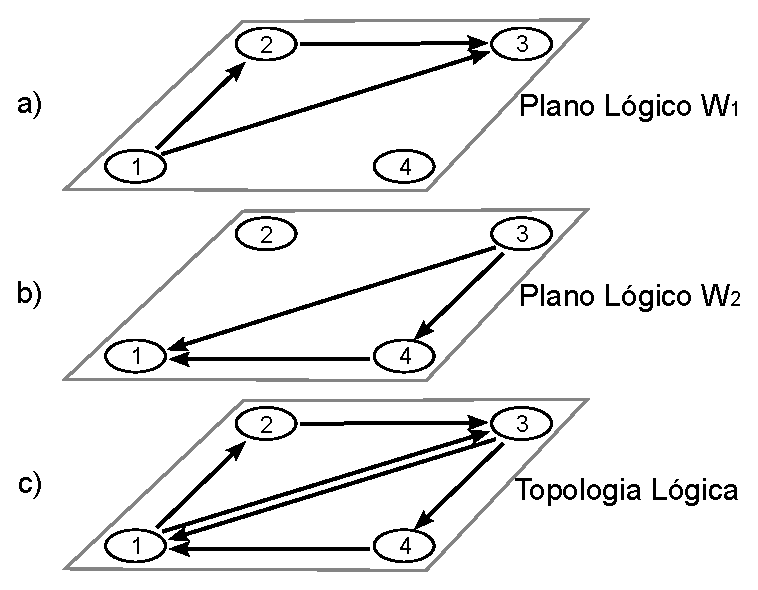
\includegraphics[bb=152 525 500 792,scale=0.7]{./figs/planos_logicos.eps}
	% planos_logicos.eps: 0x0 pixel, 300dpi, 0.00x0.00 cm, bb=152 524 442 792
	\caption{Esquema da separa��o da topologia l�gica por comprimento de onda.}
	\label{fig:planos_logicos}
\end{figure}

Essa forma de visualizar a topologia l�gica tem apenas a finalidade de facilitar a interpreta��o das restri��es,
pois permite ver o projeto como se fossem $W$ redes sem multiplexa��o sobrepostas.
Nas se��es que se seguem no restante deste cap�tulo, a separa��o da topologia l�gica por comprimento de onda ser� usada na explana��o sobre as restri��es do
modelo TWA.  

\subsection{Continuidade de Comprimentos de Onda e Capacidade}
\label{cap:twa-sec:Bconserv_Cap}

A Restri��o \ref{rest:DefCapFlow} acumula m�ltiplas fun��es, atuando como restri��o de continuidade de comprimentos de onda e limita��o de
capacidade. Em cada plano l�gico $w$, ela garante a continuidade das rotas f�sicas, onde os componentes topol�gicos devem formar uma caminho sobre a
topologia f�sica, conservando o mesmo comprimento de onda. Esses percursos n�o s�o controlados explicitamente; eles s�o garantidos pela conserva��o dos
componentes topol�gicos nos n�s intermedi�rios, semelhante a uma restri��o de conserva��o de fluxo \cite{ramamurthy99}. 

A Restri��o \ref{rest:DefCapFlow} � repetida na equa��o \ref{eq:DefCapFlow} para facilitar a leitura desta se��o. Nela, a conserva��o dos percursos l�gicos
� feita da seguinte forma: a soma dos componentes das liga��es l�gicas iniciadas em um n� $i$ no plano $w$, partindo de um n� intermedi�rio $v$, deve ser
menor ou igual � quantidade recebida. Isso � garantido se a equa��o \ref{eq:ConserB} for satisfeita.

\begin{equation}
\sum_{s} q_{sw}^{iv}\cdot A_s \leqslant Cap\cdot \left(\sum_{m} B_{iw}^{mv} - \sum_{n} B_{iw}^{vn}\right) \Forall{(i,v,w)} \mbox{, com $i\neq v$}
\label{eq:DefCapFlow}
\end{equation} 

\begin{equation}
   \sum_{n} B_{iw}^{vn} \leqslant \sum_{m} B_{iw}^{mv}  \Forall{(i,v,w)}
   \label{eq:ConserB}
\end{equation}

A equa��o \ref{eq:ConserB} pode ser reescrita na forma da equa��o \ref{eq:ConserBdif}, que define $LL^{iv}_w$, a diferen�a entre a soma dos
componentes chegando e saindo de $v$, originados em $i$ no plano $w$. O valor
$LL^{iv}_w$ representa a quantidade de liga��es l�gicas que n�o t�m continuidade ao passar por $v$, ou seja, s�o as liga��es l�gicas incidentes em $v$,
com origem em $i$ no plano $w$.

\begin{equation}
  LL^{iv}_w = \sum_{m} B_{iw}^{mv} - \sum_{n} B_{iw}^{vn} \geqslant 0 \Forall{(i,v,w)}
   \label{eq:ConserBdif}
\end{equation}

 Por sua vez, a equa��o \ref{eq:ConserBdif} � equivalente � equa��o
\ref{eq:ConserBcap}. Este �ltima � garantida pela Restri��o \ref{rest:DefCapFlow}, como fica demostrado pela equa��o \ref{eq:ConserBfim}, pois tomando-a
como premissa conclui-se a equa��o \ref{eq:ConserBcap}. Portanto, a equa��o \ref{eq:ConserB} � v�lida. 

\begin{equation}
   0  \leqslant Cap\cdot LL^{iv}_w \Forall{(i,v,w)}
   \label{eq:ConserBcap}
\end{equation}

\begin{equation}
   \sum_{s} q_{sw}^{iv}\cdot A_s  \leqslant Cap\cdot LL^{iv}_w \Forall{(i,v,w)}
   \label{eq:ConserBfim}
\end{equation}

Na figura \ref{fig:Bconserv} � ilustrada a forma como a conserva��o dos percursos l�gicos � feita. Nela v�-se dois componentes chegando no
n� intermedi�rio $v$, ambos comp�em liga��es l�gicas no plano $w$ iniciadas no n� $i$, que n�o est� representado na figura, igualmente ao componente que
deixa $v$. A soma dos valores dos componentes que chegam � $3$ e a dos que saem � $2$, portanto a conserva��o est� mantida. Neste exemplo, como h�
diferen�a de $1$ entre a quantidade de componentes chegando e saindo de $v$, ent�o, necessariamente h� $1$ liga��o l�gica terminando em $v$; para a qual
ele deixa de ser visto como um n� intermedi�rio, se tornando o destino dessa liga��o l�gica. A conserva��o n�o seria mantida no plano $w$ houvessem
componentes partindo de $v$ em maior quantidade do que chegando, pois ai n�o haveria rastreabilidade do percurso at� sua origem $i$. 
 
\begin{figure}[htb]
	\centering
	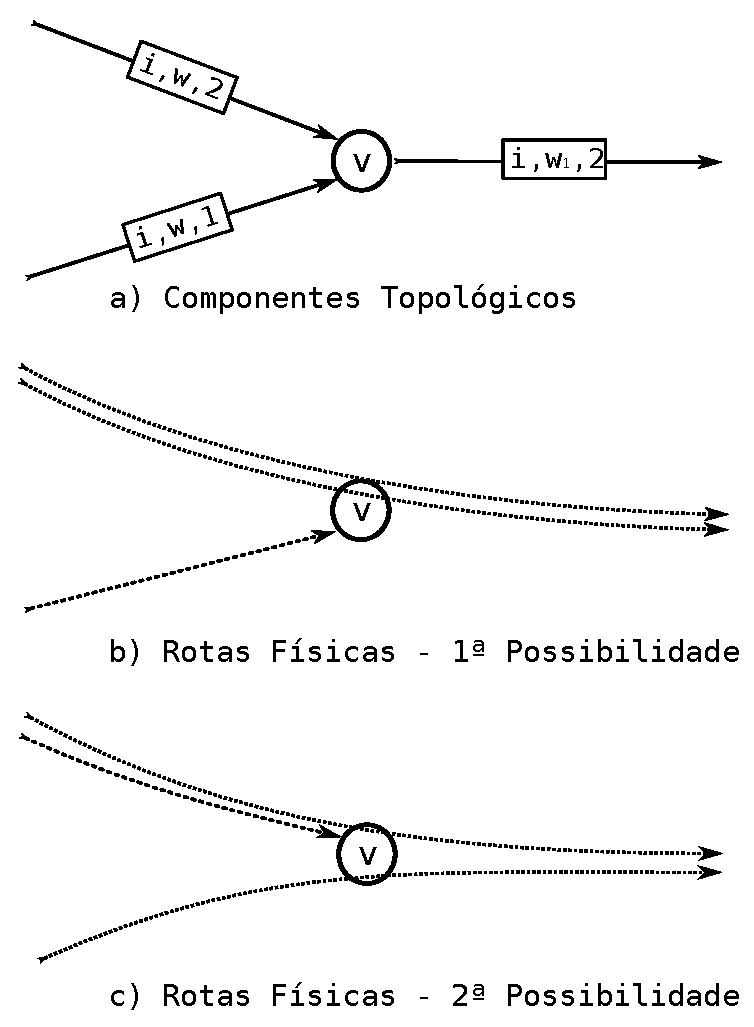
\includegraphics[bb=109 621 445 749,scale=0.7]{./figs/B_conserv.eps}
	% B_conserv.eps: 0x0 pixel, 300dpi, 0.00x0.00 cm, bb=106 272 452 749
	\caption{Conserva��o dos Percursos L�gicos.}
	\label{fig:Bconserv}
\end{figure}

A Restri��o \ref{rest:DefCapFlow} � um conjunto de equa��es, onde cada uma trata de um par $(i,j)$ em um plano l�gico $w$. Portanto, a capacidade das
liga��es l�gicas associadas ao par $(i,j)$ � a capacidade de cada uma ($Cap$) multiplicada pelo n�mero de liga��es l�gicas entre $(i,j)$ no plano l�gico
$w$.
Este segundo fator � $LL^{ij}_w$, calculado na equa��o \ref{eq:ConserBdif}. Todo o tr�fego passando pelas liga��es l�gicas $(i,j)$ nesse plano
deve ser limitado por $Cap\cdot
LL^{ij}_w$, o que de fato � feito pela Restri��o \ref{rest:DefCapFlow}. 

A Restri��o \ref{rest:DefCapFlow} ainda acumula uma fun��o que, por ser intuitiva, pode passar desapercebida, mas � fundamental para a consist�ncia do
modelo. Ela anula as fra��es de fluxo agregado entre os n�s n�o conectados diretamente por liga��es l�gicas. Quando $LL^{ij}_w = 0$, ou seja, n�o
h� liga��es l�gicas entre o par $(i,j)$ no plano $w$, as fra��es de fluxo $q_{sw}^{ij}$ ser�o anuladas pela Restri��o \ref{rest:DefCapFlow}, para todas as
origens $s$.

\subsection{Controle da Topologia F�sica}

Com a finalidade de controlar pela fun��o objetivo \ref{fo:MinC} a quantidade de liga��es f�sicas definidas pelos componentes topol�gicos, a Restri��o
\ref{rest:DefFis} acumula nas vari�veis $D_{mn}$ a multiplicidade determinada pelos componentes. Ela � repetida na
equa��o \ref{eq:DefFis} para facilitar a leitura desta se��o. Dado um par $(m,n)$, as equa��es
dessa restri��o s�o ainda separadas por comprimento de onda. Pois se todos os componentes topol�gicos alocados em $(m,n)$ usarem o mesmo $w$, apenas uma
liga��o f�sica ser� necess�ria. Se usarem comprimentos de onda diferentes, $D_{mn}$ precisar� atender ao maior desses componentes topol�gicos. Portanto, a
restri��o \ref{rest:DefFis}, minimiza a soma dos maiores de componentes topol�gicos em cada par $(m,n)$, por for�a do fator $CI$ na fun��o objetivo (Se��o
\ref{cap:twa-sec:funcaoobjetivo}).

\begin{equation}
\sum_i B_{iw}^{mn} \leqslant D_{mn} \Forall{(m,n,w)}
\label{eq:DefFis}
\end{equation} 

\begin{figure}[htb]
	\centering
	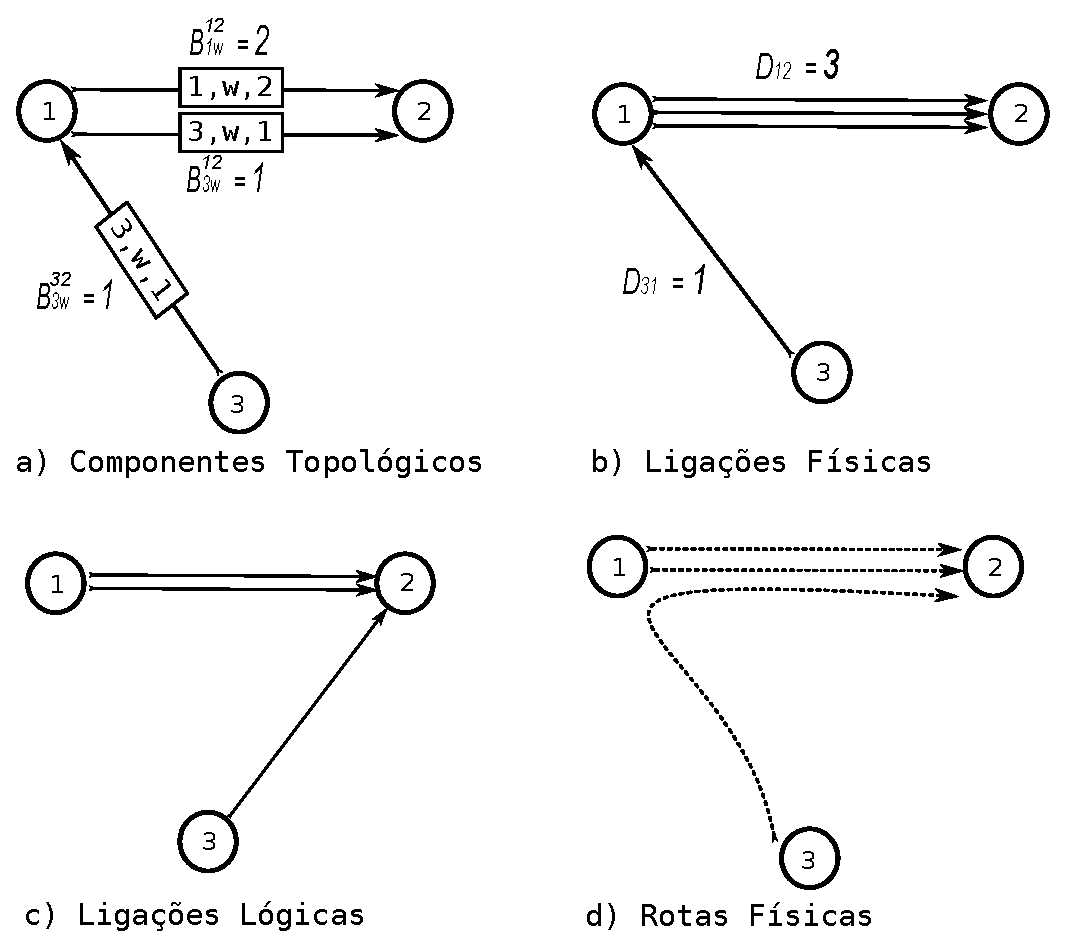
\includegraphics[bb=37 371 534 812, scale=0.7]{./figs/Var_Dmn.eps}
	% Var_Dmn.eps: 0x0 pixel, 300dpi, 0.00x0.00 cm, bb=34 593 536 800
	\caption{Interpreta��o dos componentes topol�gicos na vari�vel $D_{mn}$.}
	\label{fig:varDmn}
\end{figure}

Na Figura \ref{fig:varDmn} est� um exemplo de interpreta��o dos componentes topol�gicos na vari�vel $D_{mn}$. No item $a$ est�o os componentes topol�gicos
que definem as liga��es f�sicas indicadas no item $b$. Nos itens $c$ e $d$ est�o as liga��es l�gicas e as rotas f�sicas correspondentes.

\subsection{Conserva��o de Fluxo}

A conserva��o de fluxo � assegurada pelas Restri��es \ref{rest:ConservFlowOut} e \ref{rest:ConservFlow}, que tamb�m garantem o envio e a entrega das
demandas de tr�fego. Elas s�o repetidas nas equa��es \ref{eq:ConservFlowOut} e \ref{eq:ConservFlow} para facilitar a leitura desta se��o.  
Essas restri��es s�o semelhantes �s encontradas na modelagem agregada para o VTD \cite{ram02}. Al�m da separa��o do tr�fego por
comprimento de onda e da normaliza��o das vari�veis, como foi comentado na Se��o \ref{cap:twa-sec:VarFracFlow}, a interpreta��o das restri��es �
sutilmente diferente pois um par $(i,j)$ representa um conjunto de liga��es l�gicas. 

\begin{equation}
\sum_{jw} q_{vw}^{vj} = 1 \Forall{v} 
\label{eq:ConservFlowOut}
\end{equation} 
 
\begin{equation}
\sum_{iw} q_{sw}^{iv} - \sum_{jw} q_{sw}^{vj} = Q_{sv} \Forall{(s,v)} \mbox{, com $s\neq v$}
\label{eq:ConservFlow}
\end{equation}

Cada par $(i,j)$ � visto nas restri��es de controle de fluxo como um �nico caminho, unindo todos os planos l�gicos. Se o par representar na verdade
m�ltiplas
liga��es l�gicas, a diferen�a � que ele ter� uma capacidade maior de receber tr�fego, que � controlada pela Restri��o \ref{rest:DefCapFlow}. Deste modo,
essas restri��es funcionam da mesma forma que em \cite{ram96}. Portanto, s�o as restri��es de conserva��o de fluxo que fazem a correla��o ente os planos
l�gicos.

A Restri��o \ref{rest:ConservFlowOut} garante que todo o tr�fego originado em cada n� $v$ seja emitido para a rede, exigindo que a soma das fra��es
de tr�fego, em todos os planos l�gicos, que iniciam na origem ($i=s=v$) seja igual a $1$, ou seja, $100\%$ do tr�fego originado em $v$. 

Por sua vez, a
Restri��o \ref{rest:ConservFlow} garante que o tr�fego emitido seja encaminhado atrav�s da rede e entregue no destino. Fixada uma origem de tr�fego $s$,
para cada n� intermedi�rio $v$ ($v\neq s$) a por��o de tr�fego que deve ser entregue � $Q_{sv}$. Ela � igual � soma do tr�fego chegando por todos
os planos l�gicos $w$, vindo de qualquer n� intermedi�rio $i$, subtra�da da soma do tr�fego partindo com destino a qualquer n� $j$, em qualquer
plano $w$. O tr�fego n�o entregue em $v$ continua seguindo seu caminho pela rede at� seu destino, e deste modo � feita rastreabilidade do tr�fego at� sua
origem. Esta restri��o apenas n�o garante que o tr�fego seja emitido na origem, tarefa cumprida pela Restri��o \ref{rest:ConservFlowOut}.

O tr�fego pode ser subdividido e transportado simultaneamente por mais de uma liga��o l�gica entre o par $(i,j)$, no plano $w$. Neste caso, como as rotas
ter�o o mesmo comprimento de onda, eles n�o compartilham liga��es f�sicas ao longo do percurso. Mas essas rotas podem ainda n�o ser disjuntas, pois �
poss�vel compartilharem n�s intermedi�rios.

\section{Limita��es da Forma B�sica do TWA}

Dada a forma agregada como � feito o roteamento dos comprimentos de onda e tamb�m pela forma impl�cita do tratamento de m�ltiplas liga��es l�gicas, sem
separ�-las em vari�veis de decis�o pr�prias, algumas quest�es de menor complexidade n�o s�o decididas pelo TWA.  Na solu��o provida pelo modelo, s�o
alocados recursos suficiente para
atender ao projeto, da forma mais econ�mica poss�vel. Mas nem todos os detalhes da configura��o da rede s�o determinados.

Como ser� mostrado nesta se��o, essas omiss�es n�o
prejudicam o projeto dentro do escopo adotado. Podendo essas quest�es n�o resolvidas serem tratadas em fases posteriores do projeto a partir da solu��o
provida pelo modelo. Isso garante a simplicidade do TWA, permitindo uma modelagem com poucas restri��es e vari�veis. 

Na lista a seguir s�o enumeradas as limita��es da forma b�sica do TWA. Em seguida, cada uma ser� explicada e formas de trat�-las ser�o
sugeridas.

\begin{enumerate}
	\item Pode n�o haver uma forma �nica para configura��o das rotas f�sicas em cada plano l�gico.
	\item Podem ocorrer ciclos nas rotas f�sicas.
	\item Pode n�o ser poss�vel saber com exatid�o a dist�ncia percorrida pelo tr�fego.
	\item N�o � modelada a exata divis�o do tr�fego entre m�ltiplas liga��es l�gicas.
	\item N�o � poss�vel minimizar diretamente o congestionamento na forma b�sica do modelo.
	\item Podem haver liga��es f�sicas n�o utilizadas na solu��o.
\end{enumerate}

Como o roteamento de comprimento de onda � feito de forma agregada, podem haver mais de uma possibilidade de configura��o das rotas f�sicas em cada plano
l�gico. Na Figura \ref{fig:B_unsolved}, � mostrado um arranjo de componentes topol�gicos com duas possibilidades de interpreta��o. Necessariamente duas
liga��es l�gicas no plano $w_1$ passam transparentemente por $v_4$, enquanto uma nele termina. Ambas possibilidades de interpreta��o dos componentes s�o
v�lidas, ou seja, o TWA n�o modela o exato percurso f�sico das liga��es l�gicas em cada plano. Todavia,
isso n�o interfere na modelagem do restante do problema e n�o precisa ser resolvido nesta fase do projeto. 

De posse da solu��o provida pelo TWA, as
rotas que possu�rem alternativas de configura��o podem ser decididas levando-se em considera��o outras m�tricas n�o abordadas aqui, como por exemplo o fator
BL, que pondera tr�fego com a dist�ncia percorrida sobre a topologia f�sica \cite{Agrawal97}. Esse tratamento seria feito para cada par $(i,j)$
independente, sendo quest�es de baixa complexidade.

\begin{figure}[htb]
	\centering
	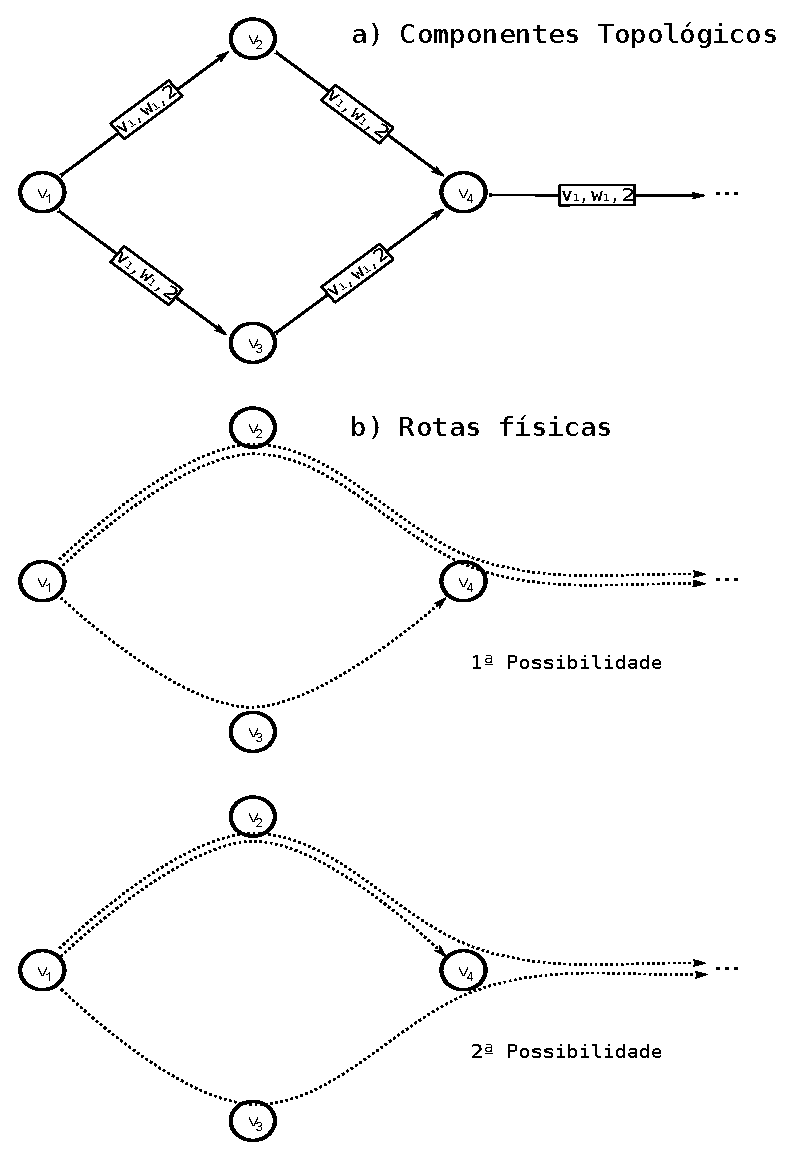
\includegraphics[bb=108 270 473 811,scale=0.7]{./figs/B_unsolved.eps}
	% B_unsolved.eps: 0x0 pixel, 300dpi, 0.00x0.00 cm, bb=108 270 473 811
	\caption{Duas possibilidades de interpreta��o dos componentes topol�gicos.}
	\label{fig:B_unsolved}
\end{figure}

Na forma b�sica do modelo TWA, podem aparecer ciclos nas rotas f�sicas, pois n�o h� esse controle no modelo b�sico. Isso poderia ser minimizado adicionando
a soma de todos os componentes topol�gicos na fun��o objetivo. Mas esses ciclos n�o interferem na modelagem e podem ser facilmente localizados e retirados
analisando a solu��o obtida.

Outra quest�o a ser determinada envolve o fato de um par $(i,j)$ poder representar m�ltiplas liga��es l�gicas. Sempre haver� banda suficiente
para atender ao tr�fego alocado respeitando � capacidade individual; isso � garantido pela Restri��o \ref{rest:DefCapFlow}. Todavia, na distribui��o do
tr�fego cada par $(i,j)$ � visto como um �nico caminho, e o tr�fego � separado apenas por comprimento de onda. O tr�fego pode ser subdividido e
transportado simultaneamente por mais de uma liga��o l�gica entre o par $(i,j)$ no plano $w$, sem compartilhar liga��es f�sicas ao longo do percurso. Mas
n�o fica definida a divis�o de tr�fego entre cada liga��o. 

A exata divis�o do tr�fego tamb�m pode ser definida em outra fase do projeto
e n�o precisa ser modelada aqui. Todavia, seria razo�vel assumir que o tr�fego fosse dividido igualmente entre as liga��es, para n�o sobrecarregar uma em
detrimento da outra. Ou poderia-se tamb�m aplicar o fator BL para fazer a divis�o do tr�fego considerando a dist�ncia percorrida. Novamente, essas
situa��es s�o pontuais, resolvendo-se para cada par $(i,j)$ individualmente sem demandar expressivo custo computacional.

Em virtude de n�o ser modelada a exata divis�o do tr�fego entre m�ltiplas liga��es l�gicas, n�o � poss�vel minimizar diretamente o
congestionamento \cite{ram02}. Mas, a capacidade das liga��es l�gicas pode exercer o papel de limitante superior (\textit{upper bound}) para o
congestionamento. Conjuntamente com a minimiza��o do tr�fego na fun��o objetivo, como foi comentado na Se��o \ref{cap:twa-sec:funcaoobjetivo}, temos uma boa
abordagem para tratar do congestionamento, como foi demostrado em \cite{Renato06}.

Por fim resta tratar da possibilidade da topologia f�sica determinada pelos componentes topol�gicos poder ser superestimada na vari�vel $D_{mn}$.
A Restri��o \ref{rest:DefFis} apenas exige que a vari�vel $D_{mn}$ seja suficiente para atender aos componentes topol�gicos, mas permite que ela assuma
valores maiores que o necess�rio. Todavia, esse poss�vel excesso n�o interfere na consist�ncia do que � modelado pelos componentes topol�gicos. Al�m disso,
ele � controlado indiretamente minimizando a fun��o objetivo, por meio do custo de instala��o, e pode ainda ser tratado analisando a solu��o fornecida,
extraindo os valores corretos diretamente dos componentes topol�gicos. A corre��o feita atrav�s da fun��o objetivo funcionaria tamb�m com qualquer outra
m�trica diretamente relacionada com a vari�vel $D_{mn}$ que fosse minimizada. 









%%%%%%%%%%%%%%%%%%%%%%%%%%%%%%%%%%%%%
%% Lower Bounds
%% Copyright 2009 Fabio de Oliveira Lima.
%% Este documento � distribu�do nos termos da licen�a 
%% GNU General Public License v2.
%%%%%%%%%%%%%%%%%%%%%%%%%%%%%%%%%%%%%


\chapter{Limitantes Inferiores}
\label{lb}


Nos trabalhos encontrados na literatura, no que diz respeito ao congestionamento, encontrar boas solu��es � uma tarefa f�cil para
heur�sticas \cite{Sivarajan01,Nina05}. Todavia, o c�lculo de limitantes inferiores (\textit{lower bounds} - LB) que garantam essa qualidade tem elevado
custo computacional, sendo esta
a parte mais dif�cil dessa abordagem. Apresentamos na se��o a seguir uma nova t�cnica para a obten��o de \textit{lower bounds} para o congestionamento. Ela
� uma formula de c�lculo direto, que denominamos \textit{Minimum Traffic Bound} (MTB), fornecendo um LB de alta qualidade para o
congestionamento, com custo computacional muito pequeno, cuja efici�ncia contrasta com as op��es encontradas na literatura \cite{ram96}. 

\section{MTB - Limitante Inferior para o Congestionamento}

Para determinar um LB para o congestionamento, precisamos estimar qual � o m�nimo de tr�fego que pode ser designado a cada liga��o l�gica da rede. N�o h�
uma
resposta direta, mas podemos fazer uma estimativa olhando cada n� independentemente. 
Na melhor das hip�teses, todo o tr�fego que passa pelas liga��es l�gicas
iniciadas em um n� $v$ � composto exclusivamente por demandas de tr�fego tamb�m originadas neste mesmo n�. Analogamente, o tr�fego nas liga��es l�gicas
incidentes em $v$ seria
composto por demandas destinadas a ele. Esses s�o os menores valores poss�veis, considerando que todo o tr�fego da rede ser� devidamente enviado e recebido.

Assim,  dividindo todo o tr�fego originado em $v$ pelo n�mero de liga��es l�gicas nele iniciadas,
temos uma estimativa do menor tr�fego poss�vel nessas liga��es l�gicas. Analogamente, uma estimativa pode ser feita para o tr�fego destinado a $v$ nas
liga��es l�gicas nele incidentes. Extrapolando isso para toda a rede, a maior dentre essas estimativas seria uma boa
candidata a limitante inferior para o congestionamento. Isto porque n�o � poss�vel que um n� envie menos tr�fego do que a soma das demandas originadas
nele. E analogamente, n�o � poss�vel que um n� receba menos tr�fego do que o destinado a ele. O MTB � assim definido como o m�nimo dos valores calculados
nas equa��es do conjunto de Dados \ref{MT}. 

Para estabelecer o MTB, consideraremos apenas o n�mero de liga��es l�gicas iniciando ou terminando em cada n� da rede. Nas modelagens para o VTD, essa � toda a
informa��o dispon�vel sobre a topologia l�gica da rede. Mas em modelagens mais abrangentes, como o TWA, isso pode n�o
ser um dado de entrada.

% {\small
\begin{dados}
Sejam $\alpha_v$ o n�mero de liga��es l�gicas originadas em um n� $v$ e $\beta_v$ o n�mero de liga��es l�gicas incidentes em $v$.
Deste modo:
\begin{enumerate}
\item $\Theta_v = \displaystyle\sum_d P_{vd}/\alpha_v\quad$ 
\item $\Gamma_v = \displaystyle\sum_s P_{sv}/\beta_v$ 
% \item $\Omega_{v_1v_2} = \max\{\Theta_{v_1},\Gamma_{v_2}\}$
\item $MTB = \max_{v_1v_2} \{\Theta_v,\Gamma_v\}$
\end{enumerate}
\label{MT}
\end{dados}

As estimativas comentadas acima, para o tr�fego m�nimo saindo e chegando em cada liga��o l�gica incidente ou originada em $v$, s�o $\Theta_v$ e $\Gamma_v$,
respectivamente. 
% Segue que, $\Omega_{v_1v_2}$ � a estimativa de tr�fego m�nimo nas liga��es l�gicas entre o par $(v_1,v_2)$, que equivale ao maior valor
% entre as estimativas de tr�fego originado em $v_1$ ($\Theta_{v_1}$) e recebido em $v_2$ ($\Gamma_{v_2}$). 
Por sua vez, o MTB � definido como o m�ximo entre as
estimativas $\Theta_v$ e $\Gamma_v$. O teorema a seguir garante que o MTB � um LB para o congestionamento. Em sua demostra��o ser� necess�ria a proposi��o
abaixo.
% estimativas $\Omega_{v_1v_2}$. O teorema a seguir garante que o MTB � um LB para o congestionamento.

\begin{proposition}
   Para qualquer solu��o vi�vel de uma inst�ncia do VTD, para cada n� $v_1$ da rede ir� existir um n� $v_2$, tal que, h� uma liga��o l�gica entre o par
$(v_1,v_2)$ na solu��o, e o tr�fego nessa liga��o � maior ou igual � $\Theta_{v_1}$. Analogamente, haver� uma liga��o entre $(v_3,v_1)$, para algum n�
$v_3$, tal que, o tr�fego nessa liga��o � maior ou igual � $\Gamma_{v_1}$ 
\end{proposition}

\begin{proof}

Seja $\Phi_{v_1v_2}$ o tr�fego em uma liga��o l�gica $(v_1,v_2)$. � necess�rio demostrar que, em uma solu��o vi�vel qualquer:

\begin{equation}
(\forall\, v_1) \,(\exists\,v_2) \mbox{, tal que, }\Phi_{v_1v_2} \geqslant \Theta_{v_1}  
\label{lb:p1}
\end{equation} 

\begin{equation}
(\forall\, v_1) \,(\exists\,v_3) \mbox{, tal que, }\Phi_{v_3v_1} \geqslant \Gamma_{v_1}  
\label{lb:p2}
\end{equation} 

Ser� provado a seguir que a afirma��o em \ref{lb:p1} � verdadeira.

Seja $\Psi_{v}$ a soma de todo o tr�fego nas liga��es l�gicas iniciadas em $v$, em uma solu��o vi�vel qualquer. O m�nimo tr�fego que $v$ pode originar,
considerando todas as liga��es l�gicas iniciadas nele, � composto pelas demandas de tr�fego com origem em $v$, ou seja, $\sum_d P_{vd}$.  Considerando que
algum tr�fego possa ser retransmitido atrav�s de $v$, apos ser processado eletronicamente, conclui-se que:

\begin{equation}
\Psi_{v} \geqslant \sum_d P_{vd}
\label{lb:traf}
\end{equation} 

Seja $\overline{\Psi}_{v}$ o tr�fego m�dio das liga��es l�gicas iniciadas em $v$, em uma solu��o vi�vel qualquer. Dividindo os dois lados da inequa��o em
\ref{lb:traf} por $\alpha_{v}$, segue que: 

\begin{equation}
\frac{1}{\alpha_v}\cdot\left(\Psi_v \geqslant \sum_d P_{vd} \right) \quad \Longrightarrow  \quad
\frac{\Psi_v}{\alpha_v} \geqslant \frac{\sum_d P_{vd}}{\alpha_v} \quad \Longrightarrow \quad
\overline{\Psi}_v \geqslant \Theta_v
\label{lb:med}
\end{equation} 
% \overline{\Psi}_{v} = \frac{\Psi_{v}}{\alpha_{v}} \geqslant \frac{\sum_d P_{{v}d}}{\alpha_{v}} = \Theta_{v}

% Portanto, $\overline{\Psi}_v \geqslant \Theta_v$; o tr�fego m�dio saindo de $v$ � maior ou igual � $\Theta_{v}$.

Como foi provado em \ref{lb:med}, para todo n�
$v_1$, $\overline{\Psi}_{v_1}\geqslant \Theta_{v_1}$, em uma solu��o vi�vel qualquer. Assim, em alguma
liga��o l�gica iniciada em $v_1$, o tr�fego � maior ou igual � $\Theta_{v_1}$, ou seja, provou-se que \ref{lb:p1} � v�lida. A demostra��o para \ref{lb:p2} �
an�loga e ser� omitida.

\end{proof}


\begin{theorem}[\textit{Minimum Traffic Bound} -- MTB]
\label{MTB} 
Dado o n�mero de liga��es l�gicas originadas e incidentes em cada n� da rede, o MTB definido no conjunto de
Dados \ref{MT} � um limitante inferior para o congestionamento.
\end{theorem}

\begin{proof}
% Seja $(\zeta,\gamma)$ uma liga��o l�gica, parte de uma solu��o �tima para o VTD, cujo tr�fego corresponde ao valor �timo do congestionamento $\lambda_max*$.
% $$\Omega_{v_1v_2} \leqslant \lambda_{max}^* \Forall{(v_1,v_2)}$$  
% Para que isso seja v�lido, � suficiente que sejam verdadeiras as inequa��es a seguir:

Seja $\lambda_{max}^*$ o valor �timo do congestionamento. Para demostrar a validade do teorema, devemos demostrar que $MTB \leqslant \lambda_{max}^*$, o que
equivale a mostrar que sejam verdadeiras as inequa��es a seguir:

\begin{equation}
\Theta_{v} \leqslant \lambda_{max}^*\Forall{v}
\label{lb:i}
\end{equation} 

\begin{equation}
\Gamma_{v} \leqslant \lambda_{max}^*\Forall{v}
\label{lb:ii}
\end{equation} 

Para demostrar que a inequa��o \ref{lb:i} � v�lida, suponha por absurdo que ela � falsa, ou seja: 

\begin{equation}
\exists\,v \mbox{, tal que, } \Theta_v > \lambda_{max}^*
\label{lb:ni}
\end{equation} 

Do que foi suposto em \ref{lb:ni}, mais da conclus�o obtida em \ref{lb:p1}, se $\Theta_{v_1} > \lambda_{max}^*$, segue que $\Phi_{v_1v_2} > \lambda_{max}^*$
para qualquer solu��o vi�vel. O que � absurdo para as solu��es �timas, pois
contraria a defini��o de $\lambda_{max}^*$, como o tr�fego da liga��o l�gica mais carregada. Isso prova que a inequa��o \ref{lb:ni} � falsa, ou seja,
demonstra que \ref{lb:i} � verdadeira, como se queria. De modo an�logo pode-se verificar a validade da inequa��o \ref{lb:ii}, que conclui a
demostra��o do teorema.
%\bsq
% O que conclui a demostra��o. 
\end{proof}

Note que n�o foi feita restri��o quanto � multiplicidade de liga��es l�gicas, nem uniformidade do grau l�gico. Estamos considerando portanto o caso mais
geral do VTD. 

Dizemos que o MTB � um LB para para o VTD, pois a �nica restri��o feita � quanto ao conhecimento do n�mero de liga��es l�gicas iniciando e terminando em cada n�.
Em modelagens mais abrangentes, como o TWA, a introdu��o de mais restri��es e vari�veis pode fazer com que o �timo do VTD se torne invi�vel. Ainda assim, o MTB
ser� um LB para o congestionamento, todavia, outras t�cnicas de obten��o de LB poderiam ser empregadas para explorar o espa�o do conjunto de solu��es que se
tornou invi�vel. Uma alternativa � a conhecida t�cnica iterativa apresentada em \cite{ram02}.

O MTB foi aqui estabelecido em sua forma mais geral, considerando que cada n� pode possuir quantidades diferentes de liga��es l�gicas originadas ou incidentes,
entretanto, na literatura � comum considerar que os n�s da rede possuem grau l�gico uniforme \cite{ram02}. Neste caso, o MTB consiste no valor m�ximo do
do conjunto das somas das demandas originadas ou recebidas em cada n�, divido pelo grau l�gico da rede.
Portanto, conv�m apresentar uma formula��o mais direcionada para implementa��es. Isso � feito a seguir no Lema \ref{lem:MTB}.

\begin{lemma}
\label{lem:MTB}
 Se a rede possui grau l�gico uniforme $GL$, o MTB pode ser definido da seguinte forma:
 $$ \mbox{MTB} = \frac{1}{GL}\cdot\max_v \left\{\sum_d P_{vd},\sum_s P_{sv}\right\}$$
\end{lemma}


Em �ltima an�lise, o MTB explora a possibilidade da liga��o l�gica mais carregada da rede transportar predominantemente tr�fego que n�o foi ou n�o ser�
retransmitido. De fato, se $(i,j)$ � a liga��o mais carregada da rede, o ideal � que a maior parte de seu tr�fego seja destinado ao n� onde onde esta
liga��o l�gica incide ($j$). Pois do contr�rio, muito tr�fego seria retransmitido ao longo da rede, congestionando outras liga��es. Isso leva a crer que o
n� $j$ pode ter muito tr�fego a receber da rede. Por outro lado, quanto mais tr�fego for origin�rio de $i$, ouve menos retransmiss�o antes de chegar nele.

Tem-se ai duas tend�ncias que podem dominar a liga��o l�gica $(i,j)$: $j$ � o destino principal na rede, ou $i$ � o principal gerador de tr�fego. �
razo�vel que uma delas prevale�a. Por exemplo, se $j$ precisa receber mais tr�fego do que $i$ origina, seria melhor $i$ escoar esse tr�fego por
outra sa�da, que n�o $j$. Estendendo essa ideia a todo o projeto da topologia l�gica � de esperar que, na solu��o �tima, grandes emissores de tr�fego
tendem a n�o iniciar uma liga��o l�gica com destino a um grande receptor de tr�fego. E mesmo quando isso ocorresse, seria razo�vel que as duas tend�ncias
n�o concorressem numa mesma liga��o l�gica, mas sim, que a mais fraca tomasse caminhos alternativos. 

Deste modo, procurar por um LB se resumiria a encontrar a tend�ncia mais forte, seja de emiss�o ou recep��o. Essa � a ideia por tr�s do MTB, que apenas
investiga a matriz de demandas de tr�fego atr�s da maior tend�ncia. Esta suposi��o revelou-se v�lida empiricamente, posto que na maioria dos testes feitos o
MTB equivale ao �timo, como ser� visto no Cap�tulo \ref{cap:testes}. Por sorte, esse comportamento tem uma rela��o t�o direta com o grau l�gico de entrada e
sa�da dos n�s. 

Mas h� um ponto fraco nessa linha de pensamento. Ela depende que o tr�fego na liga��o l�gica mais carregada seja predominantemente caracterizado por sua
tend�ncia dominante. Isso tende a ser mais certo quanto mais assim�trica for matriz de demandas. Mas, se esta for fortemente uniforme, com pouca varia��o
entre o tamanho da demandas, a quantidade de tr�fego a ser retransmitida na rede superar� com facilidade as tend�ncias individuas de cada n�. Portanto, �
esperado que a qualidade do LB fornecido pelo MTB seja melhor em cen�rios de tr�fego assim�trico. Todavia, nos testes realizados no Cap�tulo
\ref{cap:testes}, mesmo para uma matriz com demandas uniformemente distribu�das, o MTB se mostrou bem eficiente.






% \subsection{Dichotomous Search Bound}
% 
% Uma forma de se obter \textit{lower bounds} para o congestionamento foi apresentada em \cite{ram02}. Esta t�cnica consiste
% na relaxa��o do modelo MILP, adicionando um \textit{lower} \textit{bound} conhecido $\lambda_{LB}$ � defini��o do congestionamento. O congestionamento
% $\lambda_{max}$ � a quantidade de tr�fego transportada pelo enlace l�gico mais solicitado $\lambda_{ij}$, ou seja, $\lambda_{max}\geq \lambda_{ij}$, $\forall
% i,j$. Se n�o h� um caminho l�gico entre os n�s $i$ e $j$ ($b_{ij}=0$), ent�o, $\lambda_{ij}=0$. Para obten��o de um novo LB para o congestionamento, �
% acrescentada a restri��o $\lambda_{max}\geq (1-b_{ij})\lambda_{LB}$, que pode ficar como $\lambda_{max}\geq \lambda_{ij}+(1-b_{ij})\lambda_{LB}$, sem modificar
% o
% modelo MILP. Todavia, relaxando a vari�vel bin�ria $b_{ij}$, permitindo que ela varie entre zero e um, esta defini��o para o $\lambda_{max}$ pode fornecer um
% valor superior a $\lambda_{LB}$, ou no m�nimo igual, mas, ainda sendo um LB para o congestionamento. 
% 
% Entretanto, �
% poss�vel usar uma ``previs�o' para se obter LBs, usando o m�todo iterativo. Pois, no modelo relaxado do ILB, n�o � necess�rio se conhecer um LB para poder
% produzir outro superior. Se, ao inv�s de entrarmos com um LB conhecido ($\lambda_{LB}$) na defini��o do congestionamento ($\lambda_{max}$), us�ssemos um valor
% qualquer $V$. Ter�amos a restri��o: 
% 
% \begin{equation}
% \label{hmaxv}
% \lambda_{max}\geq \lambda_{ij}+(1-b_{ij})V
% \end{equation} 
% 
% Para este contexto, faremos a seguir algumas defini��es. Sejam:
% 
% \begin{itemize}
%  \item $\lambda_{max}(V)$, os $\lambda_{max}$ definidos em fun��o deste $V$.
%  \item $W(V)=\min\{\lambda_{max}(V)\}$, o m�nimo dentre os $\lambda_{max}$ no modelo MILP relaxado, definidos pelo conjunto de restri��es na Equa��o \ref{hmaxv}
% acima. Ou seja, o �timo na relaxa��o do ILB, mas com $V$ no lugar de $\lambda_{LB}$.
% \item $Z^*$, o �timo do modelo MILP para uma dada inst�ncia.
% \end{itemize}
% 
% Segue que, se $V\geq Z^*$ ent�o $W(V)\leq V$, pois, no modelo MILP, setando este $V$, o �timo seria ele mesmo. Assim, na relaxa��o esta desigualdade �
% garantida.
% Pois, relaxando um modelo de minimiza��o, abrimos a possibilidade de encontrar uma solu��o menor. Mas, um modo equivalente de se escrever esta desigualdade �:
% se
% $W(V) > V$ ent�o $V<Z^*$. Ou seja, entrando com um valor qualquer no lugar do LB, no processo iterativo, se o resultado for maior que o valor passado, ent�o ele
% era de fato um LB para aquela inst�ncia. 






%%%%%%%%%%%%%%%%%%%%%%%%%%%%%%%%%%%%%
%% Experimentos Computacionais
%% Copyright 2009 Fabio de Oliveira Lima.
%% Este documento � distribu�do nos termos da licen�a 
%% GNU General Public License v2.
%%%%%%%%%%%%%%%%%%%%%%%%%%%%%%%%%%%%%


\chapter{Experimentos Computacionais com o TWA}
\label{cap:testes}

Para avaliar a pertin�ncia desta nova abordagem, testes computacionais foram realizados. Toda a modelagem do TWA foi descrita em AMPL�
(\textit{A Modeling Language for Mathematical Programming} - www.ampl.com), de modo que facilmente 
possa ser adaptada para v�rias finalidades. Utilizamos o \textit{solver} SCIP (\textit{Solving Constraint Integer Programs} - scip.zib.de) para resolver o modelo
MILP do TWA. Para interpretar o c�digo AMPL, gerando a entrada de dados para o SCIP, foi usado o GLPK (\textit{GNU Linear Programming Kit} -
www.gnu.org/software/glpk/). Vale observar que o SCIP e o GLPK s�o \textit{softwares} livres, de c�digo fonte aberto e de distribui��o gratuita.

Os resultados dos experimentos computacionais realizados com o TWA s�o comparados, neste cap�tulo, com os
publicados em \cite{Karcius04} e \cite{Sivarajan01}, aonde foram propostos modelos para a resolu��o integrada do VTD e RWA. 

A modelagem encontrada em \cite{Karcius04} � baseada nas modelagens cl�ssicas desses problemas \cite{ram02, Zang00}, o qual denominaremos \textbf{VTD-RWA}. Este
trabalho prop�e um algoritmo iterativo, que faz uso de programa��o linear, para resolver os problemas VTD e RWA de forma integrada. A solu��o do VTD gera
requisi��es para um conjunto de caminhos, representados pela topologia virtual, que devem ser roteados pela topologia f�sica. Os caminhos s�o alocados de maneira
a minimizar crit�rios de otimiza��o. A estrat�gia foi testada para redes com caracter�sticas distintas, mas n�o sendo considerado convers�o de comprimentos de
onda.

Para os resultados publicados em \cite{Sivarajan01}, � feita uma modelagem MILP que minimiza congestionamento em redes sem conversores de comprimentos de onda, o
qual denominaremos \textbf{KS}. Segundo os autores, esta formula��o n�o � computacionalmente trat�vel, sendo m�todos heur�sticos propostos. O Modelo MILP �
relaxado e executado interativamente por $25$ vezes usando um plano de corte. As vari�veis que representam a topologia virtual e os percursos f�sicos s�o
arredondadas, enquanto uma heur�stica de aloca��o de comprimentos de onda � aplicada para atribuir comprimentos de onda individualmente aos caminhos �pticos. O
tr�fego � roteado pela topologia virtual utilizando uma formula��o linear (LP) consistindo somente das restri��es de tr�fego do MILP relaxado. Uma das
desvantagens desse m�todo � que supondo que existam $W$ comprimentos de onda dispon�veis em cada fibra, o MILP relaxado obtem uma solu��o que satisfaz esta
restri��o. No entanto, sendo que o algoritmo de aloca��o de comprimentos de onda, que � aplicado subsequentemente, obtem solu��es sub�timas, n�o h� garantia de
uma aloca��o de comprimentos de onda com sucesso, respeitando o limite de $W$ comprimentos de onda. Como resultado, o m�todo n�o retorna necessariamente solu��es
vi�veis para todos os casos. 


\section{Compara��o com o modelo VTD-RWA}
\label{cap:testes-sec:karcius}

Nos resultados que iremos confrontar, s�o considerados: o grau l�gico da rede ($Gl$), o n�mero de liga��es l�gicas em cada fibra ($L$), o n�mero de comprimentos
de onda dispon�veis em cada liga��o f�sica ($W$) e o n�mero de saltos f�sicos na topologia ($S$). Esses par�metros s�o comumente tratados nas investiga��es a
cerca do RWA \cite{Zang00}.

Tamb�m � controlado o congestionamento, que � uma conhecida m�trica para o VTD. Isso � feito atrav�s da cl�ssica heur�stica HLDA \cite{ram02,
sbpo04}, gerando uma solu��o para o VTD que alimenta as etapas seguintes do procedimento, conforme apresentado em \cite{Karcius04}. Para cada grau
l�gico, o HLDA produz de forma determin�stica uma topologia l�gica, baseado na matriz de demandas. A solu��o para o VTD � completada distribuindo o
tr�fego sobre esta topologia, atrav�s de um modelo de programa��o linear \cite{ram02}.

Para produzir resultados pass�veis de compara��o, s�o acrescentadas � modelagem b�sica do TWA, mostrada na Se��o \ref{Basic}, as restri��es de 
controle do grau l�gico (Restri��o \ref{ConservGl}) e a de limita��o do n�mero de liga��es l�gicas em cada fibra (Restri��o \ref{L}). Esta formula��o 
espec�fica � denominada de TWA-$a$. Para controlar a qualidade das solu��es quanto ao congestionamento, foram obtidas topologias virtuais com uma 
implementa��o da heur�stica HLDA. Para cada uma destas topologias, foi distribu�do o tr�fego e calculado o congestionamento atrav�s do 
\textit{solver} do \textit{software} GLPK (\textit{GNU Linear Programming Kit} - www.gnu.org/software/glpk/), utilizando uma vers�o do 
modelo cl�ssico para o VTD \cite{ram02}. O valor de congestionamento obtido, arredondado para cima, foi usado como a capacidade dos canais 
l�gicos, na Restri��o (\ref{DefCapFlow}). Para cada inst�ncia, esse procedimento levou menos de um segundo, portanto n�o ser� 
considerado na contagem de tempo de processamento dos nossos resultados.

A estrat�gia adotada foi, partindo do menor grau l�gico ($Gl=1$), fixar nos valores m�nimos o n�mero de comprimentos de onda e a limita��o de 
liga��es das fibras ($W=1$ e $L=1$), minimizando o n�mero de saltos ($S$). Um solver para problemas MILP � instanciado com essa configura��o. 
Enquanto o solver retornar que o problema � insol�vel \cite{mukherjee}, $L$ ser� incrementado at� o seu limite, que � o valor atual de $W$. Quando 
$L$ n�o puder ser aumentado ($L=W$), ent�o $W$ o ser�, e assim por diante. Se uma solu��o vi�vel � encontrada, o solver � interrompido, a solu��o
� registrada e o grau l�gico � incrementado, dando continuidade ao processo.

% Se o solver n�o encontrar uma solu��o vi�vel dentro de $400$ segundos, ent�o ele � abortado e � aplicado o mesmo precedimento de quando a
% solu��o 
% � insol�vel. Isso � feito com o objetivo de ``afrouxar'' as restri��es de modo que o solver possa encontrar uma solu��o vi�vel mais rapidamente, 
% sacrificando um pouco a qualidade das restri��es. Se uma solu��o vi�vel � encontrada, dentro da janela de $400$ segundos, o solver �
% interrompido, 
% a solu��o � registrada e o grau l�gico � incrementado, dando continuidade ao processo. 

Nas situa��es em que o problema era insol�vel, o solver determinou isso em menos de um segundo, dificultando a separa��o dos tempos de leitura e
de execu��o. Portanto estes tempos n�o foram computados. Essas situa��es em que o modelo precisou ser calibrado, que chamaremos de
\textit{Inst�ncia Insol�vel} ($I$), fazem parte do m�todo e s�o registradas conjuntamente com os resultados.

% Este arranjo n�o foi obtido ao acaso e nem por tentativa e erro. O grau l�gico ($Gl$), o n�mero de comprimentos de onda ($W$), a limita��o de 
% liga��es l�gicas das fibras ($L$), a capacidade do canal ($Cap$) e o n�mero de saltos ($S$), deveriam ser controlados para viabilizar a compara��o 
% com o trabalho do Karcius. O par�metro $S$ foi escolhido para a fun��o objetivo pois, dentre as op��es, era a que fornecia o modelo mais enxuto. 
% Al�m disso, a minimiza��o do n�mero de saltos ajuda a evitar a forma��o de ciclos na solu��o \cite{Karcius04}. 

Como, nesta modelagem, $W$ est� diretamente relacionado a quantidade de vari�veis, � mais conveniente come�ar com $W=1$. Disso decorre a escolha 
de tamb�m come�armos com $Gl=1$ e $L=1$. A maior prioridade para a incrementa��o � dada ao $Gl$, pois variando este temos inst�ncias diferentes. 
A menor preced�ncia ficou para $W$, pois quanto menor ele for menores precisar�o ser os custos de instala��o da rede. Na posi��o intermedi�ria 
fica $L$, pois, minimizando-o, maximizamos a disponibilidade da rede.

 Utilizamos o \textit{solver} SCIP (\textit{Solving Constraint Integer Programs} - scip.zib.de) para encontrar as solu��es vi�veis. Al�m de
calcular a capacidade dos canais �pticos ($Cap$), como foi descrito acima, o GLPK tamb�m foi usado para interpretar o modelo AMPL, gerando a
entrada de dados para o SCIP. Vale observar que o SCIP e o GLPK s�o \textit{softwares} livres, de c�digo fonte aberto e de distribui��o gratuita.
Os resultados que ser�o confrontados com os nossos foram produzidos com o ILOG CPLEX� (www.ilog.com/products/cplex), uma ferramenta
comercial.

Foram executados dois testes computacionais, com uma rede de $6$ n�s e com uma rede de $12$ n�s \cite{Karcius04}. Os resultados foram compilados
nas Tabelas \ref{N6} e \ref{N12}, cujas legendas est�o resumidas na Tabela \ref{tab:legendas}. Todos os testes foram executados em um \textit{notebook}
\textit{PC} (\textit{Linux Ubuntu} $8.04$, $32 bits$), equipado com processador \textit{Sempron Mobile $3500+$} ($1.8 GHz$, $512 KB$) e $2 GB$
$DDR2$ ($533 MHz$).

\begin{table}[!ht]
\begin{center}

\begin{tabular}{|ccl|} \hline
$GL$  & $ =$ & Grau L�gico\\
$L$   & $ =$ & Limita��o de Liga��es l�gicas das Fibras\\
$W$   & $ =$ & N�mero de comprimentos de onda dispon�veis\\
$S$   & $ =$ & N�mero de Saltos F�sicos\\
$t$   & $ =$ & Tempo em segundos para encontrar a primeira solu��o vi�vel\\
$Cap$ & $ =$ & Capacidade de Tr�fego de Cada Canal �ptico\\
$I$   & $ =$ & Inst�ncia Insol�vel\\ \hline
% $F$   & $ =$ & Tentativa Falha \\ \hline
\end{tabular}

\caption{Legendas para as Tabelas \ref{N6} e \ref{N12}.}

\label{tab:legendas}
\end{center}
\end{table}

Os resultados para a rede de $6$ n�s foram compilados na Tabela \ref{N6}. A primeira coluna registra o grau l�gico de cada inst�ncia ($Gl$), que 
neste caso foram $5$. Da segunda at� a quarta coluna ($L$, $W$ e $S$) est�o os resultados de \cite{Karcius04} e da quinta � s�tima est�o os 
resultados obtidos com a metodologia descrita acima.. Note que em todas as inst�ncias foram obtidos resultados melhores.

\begin{table}[!ht]
\begin{center}
\begin{tabular}{c|ccc|ccc|ccc|} %\\ \hline
    &  \multicolumn{3}{c}{VTD-RWA} \vline  & \multicolumn{6}{c}{TWA-$a$} \\ \hline
$ Gl$ & $ L$ & $W$ & $ S  $ & $ L$ & $W$ & $ S $ & $ t $ & $Cap$ & $ I $\\ \hline
$ 1 $ & $ 1$ & $1$ & $ 09 $ & $ 1$ & $1$ & $ 06*$ & $00$ & $ 08$ & $ 0 $\\
$ 2 $ & $ 2$ & $2$ & $ 18 $ & $ 1$ & $1$ & $ 11*$ & $03$ & $ 03$ & $ 0 $\\
$ 3 $ & $ 2$ & $2$ & $ 32 $ & $ 1$ & $1$ & $ 14*$ & $00$ & $ 02$ & $ 0 $\\
$ 4 $ & $ 3$ & $3$ & $ 41 $ & $ 2$ & $2$ & $ 25*$ & $10$ & $ 01$ & $ 2 $\\
$ 5 $ & $ 4$ & $5$ & $ 50 $ & $ 3$ & $3$ & $ 46*$ & $00$ & $ 01$ & $ 2 $\\ \hline \hline
\end{tabular}

\caption{Resultados para a rede de $6$ n�s. *: Solu��o �tima.}

\label{N6}
\end{center}
\end{table}


A oitava coluna da Tabela \ref{N6} traz o tempo , em segundos, que o \textit{solver} levou para encontrar a primeira solu��o vi�vel ($t$). Um fato 
importante � que em todas as inst�ncias desta bateria de testes, este tempo foi suficiente para determinar a otimalidade da solu��o vi�vel 
encontrada. Essa possibilidade, al�m do interesse te�rico, corrobora para a efici�ncia do m�todo aqui aplicado. Em  \cite{Karcius04}  n�o s�o 
encontradas solu��es �timas e n�o foi informado o tempo gasto nesta etapa.

Ainda na Tabela \ref{N6}, na nona coluna temos a capacidade do canal �ptico ($Cap$) e por fim, na �ltima coluna temos o hist�rico das tentativas 
de calibra��o do modelo, do tipo Inst�ncia Insol�vel ($I$). Nesta coluna, um \textit{zero} significa que os resultados registrados nesta mesma 
linha foram conseguidos na primeira execu��o do \textit{solver}. Analogamente, um n�mero diferente de zero significa a quantidade de vezes em que 
foram encontradas inst�ncias insol�veis, antes da execu��o que proveu o resultado expresso nesta linha. 

%Outra diferen�a � que esta tabela tr�s uma coluna a mais, a �ltima. Ela representa o hist�rico das tentativas de 
%calibra��o do modelo, do tipo Tentativa Falha ($F$). 

%  \clearpage
\begin{table}[!ht]
\begin{center}

\begin{tabular}{c|ccc|ccc|ccc} %\\ \hline
    &  \multicolumn{3}{c}{VTD-RWA} \vline& \multicolumn{6}{c}{TWA-$a$} \\ \hline
$ Gl$ & $ L$ & $W$ & $  S  $ & $ L$ & $W$ & $  S        $ & $ t  $ & $Cap$ & $ I $\\ \hline
$ 1 $ & $ 1$ & $1$ & $ 032 $ & $ 1$ & $1$ & $ 013*      $ & $016 $ & $ 35$ & $ 0 $\\
$ 2 $ & $ 2$ & $2$ & $ 052 $ & $ 1$ & $1$ & $ 027\,\,\, $ & $031 $ & $ 10$ & $ 0 $\\
$ 3 $ & $ 3$ & $3$ & $ 078 $ & $ 2$ & $2$ & $ 066\,\,\, $ & $176 $ & $ 04$ & $ 2 $\\
$ 4 $ & $ 4$ & $4$ & $ 104 $ & $ 2$ & $2$ & $ 074\,\,\, $ & $070 $ & $ 03$ & $ 0 $\\
$ 5 $ & $ 4$ & $4$ & $ 130 $ & $ 3$ & $3$ & $ 108\,\,\, $ & $133 $ & $ 02$ & $ 2 $\\
$ 6 $ & $ 5$ & $5$ & $ 147 $ & $ 3$ & $3$ & $ 091\,\,\, $ & $003 $ & $ 02$ & $ 0 $\\ \hline \hline
\end{tabular}

\caption{Resultados para a rede de $12$ n�s. *: Solu��o �tima.}

\label{N12}
\end{center}
\end{table}

Com o mesmo arranjo de colunas descrito acima, a Tabela \ref{N12} tr�s os resultados para a rede de $12$ n�s. Desta vez temos $6$ inst�ncias, do 
grau l�gico $1$ at� o $6$. Aqui tamb�m foram obtidos melhores resultados para o trio $L$, $W$ e $S$. Nesta etapa, os resultados de \cite{Karcius04}
foram obtidos com $6$ horas de execu��o, enquanto os resultados com o modelo TWA levaram $7.2$ minutos para serem produzidos. 

Mesmo quando n�o foi encontrado o valor �timo para  $S$, atrav�s do m�todo utilizado, a otimalidade est� garantida para os par�metros $L$
e $W$. Em particular, note que apenas a varia��o de $W$ influenciou nos resultados, pois $L$ sempre teve de ser fixado no seu valor m�ximo ($L =
W$).
Um detalhe importante � que, para a primeira inst�ncia da rede de $12$ n�s ($Gl=1$), o \textit{solver} tamb�m foi capaz de provar a otimalidade
para a primeira solu��o vi�vel. Isto demonstra que o modelo TWA mant�m desempenho
aceit\'avel mesmo com uma rede de maior porte. Com esses resultados mostramos
a viabilidade da t�cnica aqui proposta, t�cnica esta que � totalmente baseada no
modelo apresentado neste trabalho. 


\section{Compara��o com o modelo KS}
\label{cap:testes-sec:sivarajan}

 Nos resultados que iremos confrontar, � considerado o grau l�gico da rede ($Gl$), n�o h� multiplicidade de liga��es l�gicas e a fun��o objetivo � o
congestionamento. Para produzir resultados pass�veis de compara��o, s�o acrescentadas � modelagem b�sica do TWA, mostrada na Se��o \ref{Basic}: as Restri��es
(\ref{ConservGl}) de controle do grau l�gico; a Restri��o (\ref{ConservMl}) de controle de multiplicidade de liga��es l�gicas, com $M=1$; e a Restri��o
(\ref{Hmax}) que determina o congestionamento como fun��o objetivo. Esta formula��o espec�fica � denominada de
TWA$c_1$.
 
Nas Tabelas \ref{p1} e \ref{p2} s�o confrontados os resultados obtidos com o TWA$c_1$ e os encontrados em \cite{Sivarajan01}, com o modelo KS. Para cada grau
l�gico, s�o exibidos: na coluna MILP, o valor de congestionamento obtido executando o modelo MILP do TWA$c_1$ com o SCIP; na coluna $T$, o tempo gasto
pelo SCIP para chegar a essa solu��o; na coluna $W$, o n�mero de comprimentos de onda utilizados pelo TWA$c_1$; e na coluna MTB, o \textit{Minimum Trafic Bound}
para cada inst�ncia. Tamb�m s�o exibidos, para o modelo KS, na coluna $UB$, as melhores solu��es para o congestionamento encontradas em  \cite{Sivarajan01}, e nas
colunas $LB$ e $W$, os respectivos \textit{lower bounds} e  n�mero de comprimentos de onda utilizados pelo KS. Quando o valor de congestionamento corresponde ao
�timo da inst�ncia, ele � marcado com um asterisco.

Nos resultados para a modelagem KS, para cada inst�ncia, o
c�lculo do LB levou em m�dia 125 minutos utilizando o m�todo iterativo encontrado em \cite{ram02}. O \textit{upper bound} (UB) foi obtido por meio de uma
heur�stica, levando menos de um minuto. Portanto, a otimalidade s� p�de ser garantida nesses resultados quando o valor vi�vel encontrado era igual ao
\textit{lower bound} obtido. Esses resultados foram produzidos com a \textit{IBM's Optimization Subroutine Library (OSL)} em um computador IBM 43P/RS6000.

\begin{table}
% [!ht]
\begin{center}
\caption{Legendas para as Tabelas \ref{p1} e \ref{p2}.}

\begin{tabular}{|ccl|} \hline
$GL$  & $ =$ & Grau L�gico\\
$W$   & $ =$ & N�mero de comprimentos de onda dispon�veis\\
MTB  & $ =$ & \textit{Minimum Trafic Bound}\\
MILP & $ =$ & Resultados obtidos pelo SCIP\\
$T$   & $ =$ & Tempo em minutos gasto com o SCIP\\
KS & $ =$ & Melhores resultados com o modelo KS\\
$LB$   & $ =$ & Lower Bound para o congestionamento\\
$UB$   & $ =$ & Uper Bound para o congestionamento\\ \hline
\end{tabular}
\label{legendas}
 \end{center}
\end{table}

\begin{table}
% [!ht]
 \begin{center}
\caption{Resultados para a matriz $P1$. *: �timo alcan�ado.}
\begin{tabular}{|c|crrr|rrc|}
\hline $P1$ &    \multicolumn{4}{|c|}{TWA$c_1$}     & \multicolumn{3}{c|}{KS}   \\ \hline \hline
		  $Gl$ & $W$ & $T_{(m)}$ &   MTB    &   MILP   & $LB$     & $UB$     & $W$ \\ \hline
		  $ 2$ & $2$ & $451$     & $126.87$ & $143.66$ & $126.74$ & $145.74$ & $4$ \\ \hline
		  $ 3$ & $3$ & $221$     & $ 84.58$ & $^*84.58$& $84.58$  & $^*84.58$& $4$ \\ \hline
		  $ 4$ & $3$ & $8$       & $ 63.44$ & $69.17$  & $63.43$  & $70.02$  & $4$ \\ \hline
		  $ 5$ & $4$ & $225$     & $ 50.75$ & $50.82$  & $50.74$  & $50.94$  & $5$ \\ \hline
		  $ 6$ & $4$ & $24$      & $ 42.29$ & $43.54$  & $42.29$  & $44.39$  & $6$ \\ \hline
		  $ 7$ & $5$ & $65$      & $ 36.25$ & $^*36.25$& $36.25$  & $36.43$  & $6$ \\ \hline
		  $ 8$ & $6$ & $102$     & $ 31.72$ & $^*31.72$& $31.72$  & $31.77$  & $7$ \\ \hline
		  $ 9$ & $7$ & $131$     & $ 28.19$ & $^*28.19$& $28.19$  & $28.37$  & $9$ \\ \hline
		  $10$ & $8$ & $72$      & $ 25.37$ & $25.53$  & $25.37$  & $25.64$  & $9$ \\ \hline
		  $11$ & $9$ & $200$     & $ 23.07$ & $23.31$  & $23.00$  & $23.08$  & $11$\\ \hline
		  $12$ & $11$& $140$     & $ 21.14$ & $21.35$  & $21.27$  & $21.39$  & $12$\\ \hline
		  $13$ & $13$& $16$      & $ 19.52$ & $^*20.25$& $20.24$  & $20.25$  & $13$\\ \hline
\end{tabular}                                               
\label{p1}                                                  
 \end{center}                                              
\end{table}                                                 
                                                                                                                                                                  
                                                                                                                                                                  
                                                                                                                                                        
% \newpage
\begin{table}
% [!ht]
 \begin{center}
\caption{Resultados para a matriz $P2$. *: �timo alcan�ado.}
\begin{tabular}{|c|crrr|rrc|}
\hline $P2$ &    \multicolumn{4}{|c|}{TWA$c_1$}     & \multicolumn{3}{c|}{KS}       \\ \hline \hline
		  $Gl$ & $W$ & $T_{(m)}$ &   MTB    &    MILP    & $LB$     & $UB$      & $W$  \\ \hline
		  $ 2$ & $1$ & $152$     & $284.66$ & $^*292.31$ & $284.26$ & $389.93$  & $2$  \\ \hline
		  $ 3$ & $2$ & $4.4$     & $189.78$ & $^*189.78$ & $189.76$ & $217.80$  & $4$  \\ \hline
		  $ 4$ & $2$ & $2$       & $142.33$ & $^*142.33$ & $142.33$ & $152.99$  & $3$  \\ \hline
		  $ 5$ & $3$ & $4$       & $113.87$ & $^*113.87$ & $113.87$ & $^*113.87$& $4$  \\ \hline
		  $ 6$ & $3$ & $3.9$     & $94.89$  & $^*94.89$  & $94.89$  & $^*94.89$ & $5$  \\ \hline
		  $ 7$ & $4$ & $4.3$     & $81.33$  & $^*81.33$  & $81.33$  & $^*81.33$ & $6$  \\ \hline
		  $ 8$ & $4$ & $6.8$     & $71.17$  & $^*71.17$  & $71.17$  & $^*71.17$ & $6$  \\ \hline
		  $ 9$ & $5$ & $20.9$    & $63.26$  & $^*63.26$  & $62.15$  & $63.26$   & $9$  \\ \hline
		  $10$ & $6$ & $20.1$    & $56.93$  & $^*56.93$  & $56.93$  & $^*56.93$ & $10$ \\ \hline
		  $11$ & $6$ & $23.2$    & $51.75$  & $^*51.75$  & $51.75$  & $^*51.75$ & $10$ \\ \hline
		  $12$ & $7$ & $23.1$    & $47.44$  & $^*47.44$  & $47.44$  & $^*47.44$ & $13$ \\ \hline
		  $13$ & $7$ & $14.8$    & $43.79$  & $^*43.79$  & $43.79$  & $^*43.79$ & $13$ \\ \hline
\end{tabular}
\label{p2}
 \end{center}
\end{table}
% \clearpage

Para ambas as matrizes, foram obtidos melhores resultados com o TWA$c_1$, em compara��o com os resultados para o modelo KS, tanto para o valor de
congestionamento quanto para o n�mero de comprimentos de onda utilizados. Outro fato importante � qualidade alcan�ada pelo MTB em todas as inst�ncias,
praticamente igual ao \textit{lower bound} obtido em \cite{Sivarajan01}, mas com demanda de tempo desprez�vel. Esse � um resultado expressivo, frente aos $125$
minutos, em m�dia, gastos com o m�todo iterativo \cite{ram02}. Por fim vale ressaltar que foram obtidas solu��es �timas para $70\%$ das inst�ncias com o TWA$c_1$,
contra
$37\%$ dos resultados para o modelo KS. 

Em $62\%$ das inst�ncias, o MTB equivale ao �timo. E mesmo quando o �timo diferiu do MTB, no pior caso, o MTB ficou menos de $5\%$ abaixo do �timo. 

O tempo demandado pelo SCIP para obter os resultados aqui apresentados s�o altos, se comparados ao desempenho de heur�sticas para o congestionamento no projeto
encontradas na literatura \cite{Sivarajan01,Nina05}. Todavia, esses resultados corroboram para efici�ncia do modelo TWA. Pois, seu reduzido n�mero de vari�veis e
equa��es, possibilitou obter tais solu��es sem que para isso fosse necess�rio recorrer � heur�sticas. 
















%%%%%%%%%%%%%%%%%%%%%%%%%%%%%%%%%%%%%
%% Conclus�o
%% Copyright 2009 Marcelo de Oliveira Lima.
%% Este documento � distribu�do nos termos da licen�a 
%% GNU General Public License v2.
%%%%%%%%%%%%%%%%%%%%%%%%%%%%%%%%%%%%%


\chapter{Conclus�es}
\thispagestyle{empty}

Uma metodologia para o projeto completo de redes... foi apresentada, englobando os os problemas VTD e RWA, al�m da escolha da topologia f�sica da rede. Esta
formula��o � ... em rela��o as apresentadas na literatura e possui a vantagem de ...

Com uma complexidade computacional ...

A metodologia foi apresentado inicialmente ... contendo as restri��es e vari�veis consideradas essenciais para a resolu��o do projeto 
completo, que engloba a escolha da topologia f�sica, defini��o da topologia virtual, distribui��o de tr�fego, defini��o das rotas f�sicas e 
aloca��o dos comprimentos de onda. Nessa modelagem a fun��o objetivo adotada foi a minimiza��o do ....

Para validar experimentalmente a formula��o, foram realizados testes ..., aonde as redes consideradas possuem $xxx$, $xxx$ n�s. Os resultados obtidos
foram consideravelmente expressivos, com rela��o � qualidade das solu��es e ao desempenho computacional.

\textit{Para a rede de $14$ n�s foram feitos testes com duas matrizes de demandas de tr�fegos, que s�o inst�ncias cl�ssicas da literatura \cite{ram96}. Para
ambas
matrizes foram obtidos resultados melhores do que os encontrados na literatura para os par�metros controlados \cite{Sivarajan01}. Al�m disso, para $70\%$ das
inst�ncias foram obtidas solu��es �timas. O tempo demandado para produzir estes �ltimos resultados foi alto, em compara��o ao desempenho das heur�sticas
utilizadas na literatura \cite{Nina05}, todavia deve-se ressaltar o fato de que n�o foram utilizadas heur�sticas nem ferramentas comerciais.
}

O novo \textit{lower bound} para o tr�fego retransmitido foi introduzido neste trabalho, o \underline{\textbf{MTB}}, demostrou ser eficiente. \textit{Pois,
possui
demanda de tempo computacional desprez�vel, frente ao alto custo das t�cnicas conhecidas at� ent�o \cite{ram96}. Al�m disso, na maioria das inst�ncias em que
conseguimos provar a otimalidade ($62\%$), o MTB coincidiu com o �timo. E mesmo quando o MTB diferiu do �timo, no pior caso, ele ficou menos de $5\%$ abaixo
deste. Apenas este resultado j� muda o cen�rio para o problema VTD, tornando este um problema bem mais trat�vel. Uma vez que, obter bons resultados a partir de
heur�sticas n�o � tarefa dif�cil no VTD, conforme a literatura \cite{ram96}.}

A abrang�ncia da modelagem e o desempenho computacional obtido viabilizam, em trabalhos futuros, realizar....


\citeoption{abnt-show-options=no}
%\nocite{*}
%\bibliographystyle{abnt-alf}
%\bibliographystyle{abnt-num}
%\bibliographystyle{sbc}
\bibliography{biblio}

%\include{anexo}

%
% \pretextualchapter{}
\chapter*{Ferramentas Computacionais}
\label{cap:ferramentas}
% \newpage


As ferramentas computacionais envolvidas neste trabalho, listadas abaixo, s�o distribu�das sob licen�as de C�digo Livre (\textit{Open Source}). O c�digo
fonte $\LaTeX$ desta disserta��o e todo o trabalho desenvolvido est� dispon�vel em \url{http://code.google.com/p/twa}. 

Todas as figuras incluidas neste texto foram criadas em SVG
(\textit{Scalable Vectorial Graphics} - \url{http://w3.org/Graphics/SVG}) e convertidas para o formato EPS (\textit{Encapsulated PostScript} -
\url{http://adobe.com/products/postscript}) para posterior inclus�o no c�digo $\LaTeX$, ambos formatos abertos. A Figura \ref{fig:nsfnet}, criada pelo autor
deste
texto, est� registrada em \url{http://wikimedia.org/wiki/File:NSFNET_14nodes.svg}.

\begin{itemize}
   \item Kubuntu GNU/Linux: a vers�o 9.10 foi usada na esta��o de trabalho e a vers�o 9.04 no servidor aonde foram
executados os testes computacionais. 
\url{http://kubuntu.org}

   \item GLPK 4.37 - \textit{GNU Linear Programming Kit}: usado para resolver modelos de programa��o inteira e converter c�digo AMPL em FreeMPS.
\url{http://gnu.org/software/glpk}

   \item SCIP - \textit{Solving Constraint Integer Programs}, vers�o 1.1.0 Linux X86: usado para resolver os modelos de programa��o interira mista.
\url{http://scip.zib.de}

   \item CLP 1.11 - \textit{Coin-or Linear Programming}: usado internamente pelo SCIP para resolver subproblemas de programa��o linear.
\url{http://coin-or.org}

   \item TexLive 2007: distribui��o $\LaTeX$ utilizada para a confec��o desta disserta��o.\\
\url{http://tug.org/texlive}

   \item Kile 2.0.83: editor de texto com ferramentas para autoria em $\LaTeX$ utilizado. \\
\url{http://kile.sourceforge.net}

   \item Inkscape 0.47: editor de desenho vetorial utilizado para criar as figuras SVG e convert�-las em EPS. 
\url{http://inkscape.org}

\end{itemize}
 

% \vspace{2cm}
% \vspace{5cm}

\begin{center}
\textbf{Feito em} \\
\textbf{$\LaTeX$}
\end{center}


\end{document}

